\documentclass[twoside]{book}

% Packages required by doxygen
\usepackage{fixltx2e}
\usepackage{calc}
\usepackage{doxygen}
\usepackage[export]{adjustbox} % also loads graphicx
\usepackage{graphicx}
\usepackage[utf8]{inputenc}
\usepackage{makeidx}
\usepackage{multicol}
\usepackage{multirow}
\PassOptionsToPackage{warn}{textcomp}
\usepackage{textcomp}
\usepackage[nointegrals]{wasysym}
\usepackage[table]{xcolor}

% NLS support packages
\usepackage[T2A]{fontenc}
\usepackage[russian]{babel}

% Font selection
\usepackage[T1]{fontenc}
\usepackage[scaled=.90]{helvet}
\usepackage{courier}
\usepackage{amssymb}
\usepackage{sectsty}
\renewcommand{\familydefault}{\sfdefault}
\allsectionsfont{%
  \fontseries{bc}\selectfont%
  \color{darkgray}%
}
\renewcommand{\DoxyLabelFont}{%
  \fontseries{bc}\selectfont%
  \color{darkgray}%
}
\newcommand{\+}{\discretionary{\mbox{\scriptsize$\hookleftarrow$}}{}{}}

% Page & text layout
\usepackage{geometry}
\geometry{%
  a4paper,%
  top=2.5cm,%
  bottom=2.5cm,%
  left=2.5cm,%
  right=2.5cm%
}
\tolerance=750
\hfuzz=15pt
\hbadness=750
\setlength{\emergencystretch}{15pt}
\setlength{\parindent}{0cm}
\setlength{\parskip}{3ex plus 2ex minus 2ex}
\makeatletter
\renewcommand{\paragraph}{%
  \@startsection{paragraph}{4}{0ex}{-1.0ex}{1.0ex}{%
    \normalfont\normalsize\bfseries\SS@parafont%
  }%
}
\renewcommand{\subparagraph}{%
  \@startsection{subparagraph}{5}{0ex}{-1.0ex}{1.0ex}{%
    \normalfont\normalsize\bfseries\SS@subparafont%
  }%
}
\makeatother

% Headers & footers
\usepackage{fancyhdr}
\pagestyle{fancyplain}
\fancyhead[LE]{\fancyplain{}{\bfseries\thepage}}
\fancyhead[CE]{\fancyplain{}{}}
\fancyhead[RE]{\fancyplain{}{\bfseries\leftmark}}
\fancyhead[LO]{\fancyplain{}{\bfseries\rightmark}}
\fancyhead[CO]{\fancyplain{}{}}
\fancyhead[RO]{\fancyplain{}{\bfseries\thepage}}
\fancyfoot[LE]{\fancyplain{}{}}
\fancyfoot[CE]{\fancyplain{}{}}
\fancyfoot[RE]{\fancyplain{}{\bfseries\scriptsize Создано системой Doxygen }}
\fancyfoot[LO]{\fancyplain{}{\bfseries\scriptsize Создано системой Doxygen }}
\fancyfoot[CO]{\fancyplain{}{}}
\fancyfoot[RO]{\fancyplain{}{}}
\renewcommand{\footrulewidth}{0.4pt}
\renewcommand{\chaptermark}[1]{%
  \markboth{#1}{}%
}
\renewcommand{\sectionmark}[1]{%
  \markright{\thesection\ #1}%
}

% Indices & bibliography
\usepackage{natbib}
\usepackage[titles]{tocloft}
\setcounter{tocdepth}{3}
\setcounter{secnumdepth}{5}
\makeindex

% Hyperlinks (required, but should be loaded last)
\usepackage{ifpdf}
\ifpdf
  \usepackage[pdftex,pagebackref=true]{hyperref}
\else
  \usepackage[ps2pdf,pagebackref=true]{hyperref}
\fi
\hypersetup{%
  colorlinks=true,%
  linkcolor=blue,%
  citecolor=blue,%
  unicode%
}

% Custom commands
\newcommand{\clearemptydoublepage}{%
  \newpage{\pagestyle{empty}\cleardoublepage}%
}

\usepackage{caption}
\captionsetup{labelsep=space,justification=centering,font={bf},singlelinecheck=off,skip=4pt,position=top}

%===== C O N T E N T S =====

\begin{document}

% Titlepage & ToC
\hypersetup{pageanchor=false,
             bookmarksnumbered=true,
             pdfencoding=unicode
            }
\pagenumbering{roman}
\begin{titlepage}
\vspace*{7cm}
\begin{center}%
{\Large Graphic Creator \\[1ex]\large 1.\+1 }\\
\vspace*{1cm}
{\large Создано системой Doxygen 1.8.11}\\
\end{center}
\end{titlepage}
\clearemptydoublepage
\tableofcontents
\clearemptydoublepage
\pagenumbering{arabic}
\hypersetup{pageanchor=true}

%--- Begin generated contents ---
\chapter{Титульная страница}
\label{index}\hypertarget{index}{}\subsection*{Титульная страница по проекту программы для создания графиков }

Пользователь обладает возможностью указывать координаты точек как с помощью ввода значений с клавиатуры, так и с помощью нажатия мышью в определенном месте на главном поле для построения. Все действия отображаются в toolbar главного окна программы. Пользователь имеет возможность добавлять кривые, указав название, цвет, толщину. Но главное – есть возможность построения нескольких кривых на одном графике. Название, цвет кривых указываются в легенде главного поля. Чтобы выбрать с какой кривой работать, пользователь имеет возможность обратиться к одной из созданных в combobox. Также можно удалять кривую, выбрав в Menu\+Bar опцию удаления. Удалять пользователь может и по одной точке. Для этого необходимо выбрать точку для удаления при помощи стрелок перемещения по графику. На главном окне программы присутствует меню для открытия, сохраниние файла. Сохранение файла производится в файлы двух расширений\+: .doc / .txt по выбору. Открытие также реализовано для двух форматов. Для ориентации по документации есть меню слева.~\newline
Основные возможности\+:~\newline
1) создавать управляемые прямые~\newline
2) определять координаты выбранной точки путем нажатия на график~\newline
3) сохранять прямые в файлы разных форматов~\newline
4) загружать прямые из файлов разных форматов~\newline
5) возможность выбрать ближайшую точку активной кривой путем нажатия на график рядом с этой точкой~\newline
6) реализован G\+UI~\newline
~\newline
~\newline
~\newline
~\newline
~\newline
~\newline
~\newline
~\newline
~\newline
~\newline
~\newline
~\newline
~\newline
~\newline
~\newline
~\newline
~\newline
~\newline
 За сим откланяюсь.~\newline
 С уважением, Silence~\newline

\chapter{Иерархический список классов}
\section{Иерархия классов}
Иерархия классов.\begin{DoxyCompactList}
\item \contentsline{section}{graph}{\pageref{classgraph}}{}
\item Q\+Dialog\begin{DoxyCompactList}
\item \contentsline{section}{My\+Delete\+Curve}{\pageref{class_my_delete_curve}}{}
\item \contentsline{section}{My\+New\+Curve}{\pageref{class_my_new_curve}}{}
\end{DoxyCompactList}
\item Q\+Main\+Window\begin{DoxyCompactList}
\item \contentsline{section}{Main\+Window}{\pageref{class_main_window}}{}
\end{DoxyCompactList}
\end{DoxyCompactList}

\chapter{Алфавитный указатель классов}
\section{Классы}
Классы с их кратким описанием.\begin{DoxyCompactList}
\item\contentsline{section}{\hyperlink{class_doc}{Doc} \\*Класс для работы с .doc форматом }{\pageref{class_doc}}{}
\item\contentsline{section}{\hyperlink{class_format_factory}{Format\+Factory} \\*The \hyperlink{class_format_factory}{Format\+Factory} class }{\pageref{class_format_factory}}{}
\item\contentsline{section}{\hyperlink{classgraph}{graph} \\*The graph class }{\pageref{classgraph}}{}
\item\contentsline{section}{\hyperlink{class_main_window}{Main\+Window} \\*The \hyperlink{class_main_window}{Main\+Window} class }{\pageref{class_main_window}}{}
\item\contentsline{section}{\hyperlink{class_my_delete_curve}{My\+Delete\+Curve} \\*The \hyperlink{class_my_delete_curve}{My\+Delete\+Curve} class }{\pageref{class_my_delete_curve}}{}
\item\contentsline{section}{\hyperlink{class_my_new_curve}{My\+New\+Curve} \\*The \hyperlink{class_my_new_curve}{My\+New\+Curve} class }{\pageref{class_my_new_curve}}{}
\item\contentsline{section}{\hyperlink{class_txt}{Txt} \\*Класс для работы с .txt форматом }{\pageref{class_txt}}{}
\end{DoxyCompactList}

\chapter{Список файлов}
\section{Файлы}
Полный список документированных файлов.\begin{DoxyCompactList}
\item\contentsline{section}{/home/silence/workplace/\+U\+I/c\+\_\+plus/{\bfseries main.\+cpp} }{\pageref{main_8cpp}}{}
\item\contentsline{section}{/home/silence/workplace/\+U\+I/c\+\_\+plus/{\bfseries mainwindow.\+cpp} }{\pageref{mainwindow_8cpp}}{}
\item\contentsline{section}{/home/silence/workplace/\+U\+I/c\+\_\+plus/\hyperlink{mainwindow_8h}{mainwindow.\+h} \\*Загловочный файл содержащий класс прямой и главное окно , в котором и рисуются прямые }{\pageref{mainwindow_8h}}{}
\item\contentsline{section}{/home/silence/workplace/\+U\+I/c\+\_\+plus/{\bfseries mydialogcurve.\+cpp} }{\pageref{mydialogcurve_8cpp}}{}
\item\contentsline{section}{/home/silence/workplace/\+U\+I/c\+\_\+plus/\hyperlink{mydialogcurve_8h}{mydialogcurve.\+h} \\*Загловочный файл окон добавления и удаления графиков }{\pageref{mydialogcurve_8h}}{}
\item\contentsline{section}{/home/silence/workplace/\+U\+I/c\+\_\+plus/{\bfseries workwithfiles.\+cpp} }{\pageref{workwithfiles_8cpp}}{}
\item\contentsline{section}{/home/silence/workplace/\+U\+I/c\+\_\+plus/\hyperlink{workwithfiles_8h}{workwithfiles.\+h} \\*Загловочный файл содержащий классы работы с файлами }{\pageref{workwithfiles_8h}}{}
\end{DoxyCompactList}

\chapter{Классы}
\hypertarget{class_doc}{}\section{Класс Doc}
\label{class_doc}\index{Doc@{Doc}}


Класс для работы с .doc форматом  




{\ttfamily \#include $<$workwithfiles.\+h$>$}



Граф наследования\+:Doc\+:\nopagebreak
\begin{figure}[H]
\begin{center}
\leavevmode
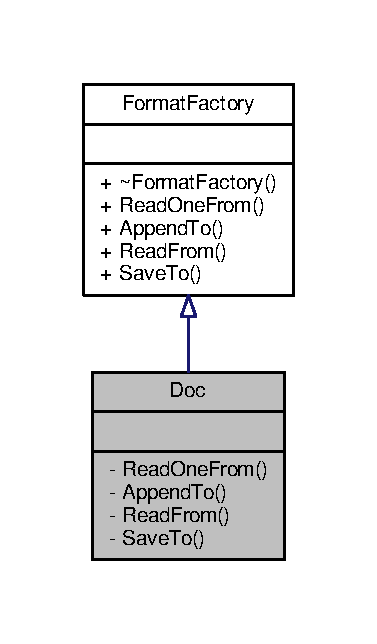
\includegraphics[width=181pt]{class_doc__inherit__graph}
\end{center}
\end{figure}


Граф связей класса Doc\+:\nopagebreak
\begin{figure}[H]
\begin{center}
\leavevmode
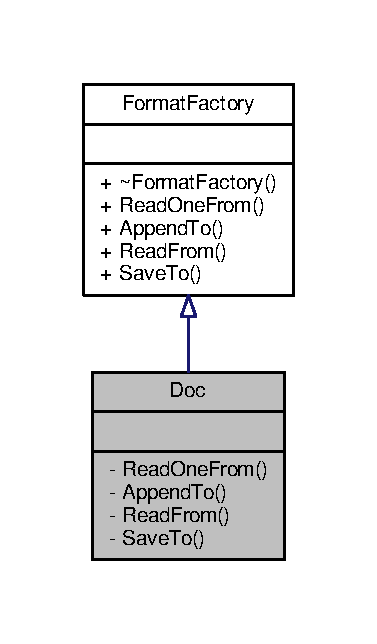
\includegraphics[width=181pt]{class_doc__coll__graph}
\end{center}
\end{figure}
\subsection*{Закрытые члены}
\begin{DoxyCompactItemize}
\item 
void \hyperlink{class_doc_a3706c27d55dbb3fe7356a6b5dbb72b5c}{Read\+One\+From} (bool \&flag, Q\+File \&file, \hyperlink{classgraph}{graph} \&FF)
\begin{DoxyCompactList}\small\item\em Читает одну прямую из .doc формата \end{DoxyCompactList}\item 
void \hyperlink{class_doc_af5c9529b9108d9155b0d725f066b3d67}{Append\+To} (bool \&flag, Q\+File \&file, \hyperlink{classgraph}{graph} \&FF)
\begin{DoxyCompactList}\small\item\em Функция сохранения одной прямой в конец файла .doc. \end{DoxyCompactList}\item 
void \hyperlink{class_doc_aa9359b8e110d9d26bcd25b68e1001743}{Read\+From} (bool \&flag, Q\+File \&file, Q\+Vector$<$ \hyperlink{classgraph}{graph} $>$ \&FF)
\begin{DoxyCompactList}\small\item\em Читает все прямые из .doc формата \end{DoxyCompactList}\item 
void \hyperlink{class_doc_a00303c942160d3e6f69b38e387f12a03}{Save\+To} (bool \&flag, Q\+File \&file, Q\+Vector$<$ \hyperlink{classgraph}{graph} $>$ \&FF)
\begin{DoxyCompactList}\small\item\em Функция сохранения в формат .doc. \end{DoxyCompactList}\end{DoxyCompactItemize}
\subsection*{Дополнительные унаследованные члены}


\subsection{Подробное описание}
Класс для работы с .doc форматом 

См. определение в файле workwithfiles.\+h строка 122



\subsection{Методы}
\index{Doc@{Doc}!Append\+To@{Append\+To}}
\index{Append\+To@{Append\+To}!Doc@{Doc}}
\subsubsection[{\texorpdfstring{Append\+To(bool \&flag, Q\+File \&file, graph \&\+F\+F)}{AppendTo(bool &flag, QFile &file, graph &FF)}}]{\setlength{\rightskip}{0pt plus 5cm}void Doc\+::\+Append\+To (
\begin{DoxyParamCaption}
\item[{bool \&}]{flag, }
\item[{Q\+File \&}]{file, }
\item[{{\bf graph} \&}]{FF}
\end{DoxyParamCaption}
)\hspace{0.3cm}{\ttfamily [private]}, {\ttfamily [virtual]}}\hypertarget{class_doc_af5c9529b9108d9155b0d725f066b3d67}{}\label{class_doc_af5c9529b9108d9155b0d725f066b3d67}


Функция сохранения одной прямой в конец файла .doc. 


\begin{DoxyParams}{Аргументы}
{\em flag} & показатель записи 1 -\/ записано 0 -\/нет \\
\hline
{\em file} & ссылка на файл \\
\hline
{\em FF} & ссылка на нужную прямую \\
\hline
\end{DoxyParams}


Замещает \hyperlink{class_format_factory_ae29ad79ca214f944962094487e668c8c}{Format\+Factory}.



См. определение в файле workwithfiles.\+cpp строка 163



Перекрестные ссылки graph\+::blue, graph\+::green, graph\+::name, graph\+::pen, graph\+::red и graph\+::tchk.



Используется в Main\+Window\+::on\+\_\+action\+Save\+\_\+current\+\_\+curve\+\_\+as\+\_\+triggered() и Main\+Window\+::on\+\_\+action\+Save\+\_\+current\+\_\+curve\+\_\+triggered().


\begin{DoxyCode}
164 \{
165     QTextStream out(&file);
166     out << FF.\hyperlink{classgraph_abfbbdbd09b20d6ef147ee966b1325595}{name} << \textcolor{stringliteral}{"\(\backslash\)t"} << FF.\hyperlink{classgraph_aa3334acd551b2fc61901c2afdd4b2d8f}{red} << \textcolor{stringliteral}{"\(\backslash\)t"} << FF.\hyperlink{classgraph_abb30b4156f98b6e0046f7192c389e4e4}{green} << \textcolor{stringliteral}{"\(\backslash\)t"} << FF.
      \hyperlink{classgraph_a2007891f138555cc8be9ca822b9fa2db}{blue} << \textcolor{stringliteral}{"\(\backslash\)t"} << FF.\hyperlink{classgraph_a237fa656ed0f8909b8eadd22aaeff422}{pen} << \textcolor{stringliteral}{"\(\backslash\)n"};
167     \textcolor{keywordflow}{for}(\textcolor{keywordtype}{int} j=0; j<FF.\hyperlink{classgraph_afae7c6852c8de983693fb2fd108ed3c4}{tchk}.size();j++)
168             out<<FF.\hyperlink{classgraph_afae7c6852c8de983693fb2fd108ed3c4}{tchk}[j].x()<<\textcolor{stringliteral}{"\(\backslash\)t"}<<FF.\hyperlink{classgraph_afae7c6852c8de983693fb2fd108ed3c4}{tchk}[j].y()<<\textcolor{stringliteral}{"\(\backslash\)n"};
169     flag=\textcolor{keyword}{true};
170 
171 \}
\end{DoxyCode}


Граф вызова функции\+:\nopagebreak
\begin{figure}[H]
\begin{center}
\leavevmode
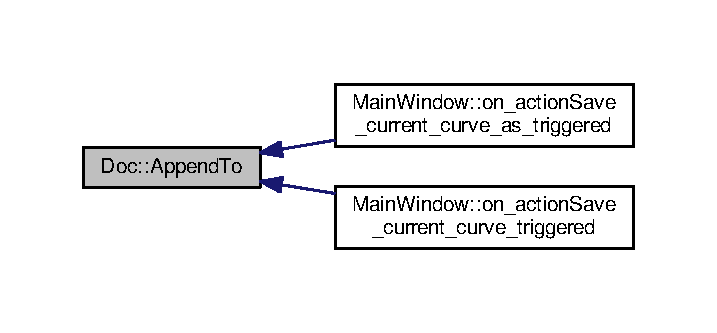
\includegraphics[width=344pt]{class_doc_af5c9529b9108d9155b0d725f066b3d67_icgraph}
\end{center}
\end{figure}


\index{Doc@{Doc}!Read\+From@{Read\+From}}
\index{Read\+From@{Read\+From}!Doc@{Doc}}
\subsubsection[{\texorpdfstring{Read\+From(bool \&flag, Q\+File \&file, Q\+Vector$<$ graph $>$ \&\+F\+F)}{ReadFrom(bool &flag, QFile &file, QVector< graph > &FF)}}]{\setlength{\rightskip}{0pt plus 5cm}void Doc\+::\+Read\+From (
\begin{DoxyParamCaption}
\item[{bool \&}]{flag, }
\item[{Q\+File \&}]{file, }
\item[{Q\+Vector$<$ {\bf graph} $>$ \&}]{FF}
\end{DoxyParamCaption}
)\hspace{0.3cm}{\ttfamily [private]}, {\ttfamily [virtual]}}\hypertarget{class_doc_aa9359b8e110d9d26bcd25b68e1001743}{}\label{class_doc_aa9359b8e110d9d26bcd25b68e1001743}


Читает все прямые из .doc формата 

\begin{DoxyWarning}{Предупреждения}
Прямые должны быть оформлены соответственно.~\newline
смотрите \hyperlink{class_doc_a00303c942160d3e6f69b38e387f12a03}{Doc\+::\+Save\+To()}; 
\end{DoxyWarning}

\begin{DoxyParams}{Аргументы}
{\em flag} & удачно ли было проведено чтение 1 -\/ да 0 -\/нет \\
\hline
{\em file} & ссылка на файл \\
\hline
{\em FF} & промежуточный вектор с прямыми \\
\hline
\end{DoxyParams}


Замещает \hyperlink{class_format_factory_ad3136c43b27e86cf755106381081e67c}{Format\+Factory}.



См. определение в файле workwithfiles.\+cpp строка 97



Перекрестные ссылки graph\+::blue, graph\+::green, graph\+::name, graph\+::pen и graph\+::red.


\begin{DoxyCode}
98 \{
99     \textcolor{keyword}{class }\hyperlink{classgraph}{graph} nov;
100     QTextStream in(&file);
101     \textcolor{keywordtype}{int} i=-1;
102     \textcolor{keywordflow}{while}(1)
103     \{
104         QString buf;
105         buf=in.readLine();
106         QStringList lst = buf.split(\textcolor{stringliteral}{"\(\backslash\)t"});
107         \textcolor{keywordflow}{if}(lst.size()==5)
108         \{
109             nov.name=lst.at(0);
110             nov.red=lst.at(1).toInt();
111             nov.green=lst.at(2).toInt();
112             nov.blue=lst.at(3).toInt();
113             nov.pen=lst.at(4).toDouble();
114             FF.push\_back(nov);
115             i++;
116         \}
117         \textcolor{keywordflow}{else} \textcolor{keywordflow}{if}(lst.size()==2)
118         \{
119             FF[i].tchk.push\_back(QPointF(lst.at(0).toDouble(),lst.at(1).toDouble()));
120         \}
121         \textcolor{keywordflow}{if}(buf.isEmpty() && lst.size()<=1)
122         \{
123             flag=\textcolor{keyword}{true};
124             \textcolor{keywordflow}{break};
125         \}
126     \}
127 \}
\end{DoxyCode}
\index{Doc@{Doc}!Read\+One\+From@{Read\+One\+From}}
\index{Read\+One\+From@{Read\+One\+From}!Doc@{Doc}}
\subsubsection[{\texorpdfstring{Read\+One\+From(bool \&flag, Q\+File \&file, graph \&\+F\+F)}{ReadOneFrom(bool &flag, QFile &file, graph &FF)}}]{\setlength{\rightskip}{0pt plus 5cm}void Doc\+::\+Read\+One\+From (
\begin{DoxyParamCaption}
\item[{bool \&}]{flag, }
\item[{Q\+File \&}]{file, }
\item[{{\bf graph} \&}]{FF}
\end{DoxyParamCaption}
)\hspace{0.3cm}{\ttfamily [private]}, {\ttfamily [virtual]}}\hypertarget{class_doc_a3706c27d55dbb3fe7356a6b5dbb72b5c}{}\label{class_doc_a3706c27d55dbb3fe7356a6b5dbb72b5c}


Читает одну прямую из .doc формата 

\begin{DoxyWarning}{Предупреждения}
Прямые должны быть оформлены соответственно.~\newline
смотрите \hyperlink{class_doc_a00303c942160d3e6f69b38e387f12a03}{Doc\+::\+Save\+To()}; 
\end{DoxyWarning}

\begin{DoxyParams}{Аргументы}
{\em flag} & удачно ли было проведено чтение 1 -\/ да 0 -\/нет \\
\hline
{\em file} & ссылка на файл \\
\hline
{\em FF} & промежуточный вектор с прямыми \\
\hline
\end{DoxyParams}


Замещает \hyperlink{class_format_factory_a0002fa7430aefd926ac94c38155b146e}{Format\+Factory}.



См. определение в файле workwithfiles.\+cpp строка 141



Перекрестные ссылки graph\+::blue, graph\+::green, graph\+::name, graph\+::pen, graph\+::red и graph\+::tchk.


\begin{DoxyCode}
142 \{
143     QTextStream in(&file);
144     QString buf;
145     buf=in.readLine();
146     QStringList lst = buf.split(\textcolor{stringliteral}{"\(\backslash\)t"});
147     FF.\hyperlink{classgraph_abfbbdbd09b20d6ef147ee966b1325595}{name}=lst.at(0);
148     FF.\hyperlink{classgraph_aa3334acd551b2fc61901c2afdd4b2d8f}{red}=lst.at(1).toInt();
149     FF.\hyperlink{classgraph_abb30b4156f98b6e0046f7192c389e4e4}{green}=lst.at(2).toInt();
150     FF.\hyperlink{classgraph_a2007891f138555cc8be9ca822b9fa2db}{blue}=lst.at(3).toInt();
151     FF.\hyperlink{classgraph_a237fa656ed0f8909b8eadd22aaeff422}{pen}=lst.at(4).toDouble();
152     \textcolor{keywordflow}{while}(1)
153     \{
154         buf=in.readLine();
155         QStringList lst1;
156         lst1=buf.split(\textcolor{stringliteral}{"\(\backslash\)t"});
157         \textcolor{keywordflow}{if}((buf.isEmpty() && lst1.size()<=1) || lst1.size()==5)
158             \textcolor{keywordflow}{break};
159         FF.\hyperlink{classgraph_afae7c6852c8de983693fb2fd108ed3c4}{tchk}.push\_back(QPointF(lst1.at(0).toDouble(),lst1.at(1).toDouble()));
160     \}
161     flag=\textcolor{keyword}{true};
162 \}
\end{DoxyCode}
\index{Doc@{Doc}!Save\+To@{Save\+To}}
\index{Save\+To@{Save\+To}!Doc@{Doc}}
\subsubsection[{\texorpdfstring{Save\+To(bool \&flag, Q\+File \&file, Q\+Vector$<$ graph $>$ \&\+F\+F)}{SaveTo(bool &flag, QFile &file, QVector< graph > &FF)}}]{\setlength{\rightskip}{0pt plus 5cm}void Doc\+::\+Save\+To (
\begin{DoxyParamCaption}
\item[{bool \&}]{flag, }
\item[{Q\+File \&}]{file, }
\item[{Q\+Vector$<$ {\bf graph} $>$ \&}]{FF}
\end{DoxyParamCaption}
)\hspace{0.3cm}{\ttfamily [private]}, {\ttfamily [virtual]}}\hypertarget{class_doc_a00303c942160d3e6f69b38e387f12a03}{}\label{class_doc_a00303c942160d3e6f69b38e387f12a03}


Функция сохранения в формат .doc. 

\begin{DoxyWarning}{Предупреждения}
Важен определенный формат расположения , а именно \+: ~\newline
Имя прямой \textquotesingle{}T\+AB\textquotesingle{} Красный цвет \textquotesingle{}T\+AB\textquotesingle{} Зеленый цвет \textquotesingle{}T\+AB\textquotesingle{} Синий цвет \textquotesingle{}T\+AB\textquotesingle{} Толщина~\newline
Координата x \textquotesingle{}T\+AB\textquotesingle{} Координата y 
\end{DoxyWarning}

\begin{DoxyParams}{Аргументы}
{\em flag} & определяет удачна ли была запись 1 -\/ да 0 -\/ нет \\
\hline
{\em file} & ссылка на файл \\
\hline
{\em FF} & все прямые для записи \\
\hline
\end{DoxyParams}


Замещает \hyperlink{class_format_factory_ac787363aa133a274ae674526dcc2b301}{Format\+Factory}.



См. определение в файле workwithfiles.\+cpp строка 128



Перекрестные ссылки graph\+::tchk.


\begin{DoxyCode}
129 \{
130     QTextStream out(&file);
131     \textcolor{keywordflow}{for}(\textcolor{keywordtype}{int} i=0; i<FF.size(); i++)
132     \{
133         out << FF[i].name << \textcolor{stringliteral}{"\(\backslash\)t"} << FF[i].red << \textcolor{stringliteral}{"\(\backslash\)t"} << FF[i].green
134             << \textcolor{stringliteral}{"\(\backslash\)t"} << FF[i].blue << \textcolor{stringliteral}{"\(\backslash\)t"} << FF[i].pen << \textcolor{stringliteral}{"\(\backslash\)n"};
135         \textcolor{keywordflow}{for}(\textcolor{keywordtype}{int} j=0; j<FF[i].tchk.size();j++)
136             out<<FF[i].\hyperlink{classgraph_afae7c6852c8de983693fb2fd108ed3c4}{tchk}[j].x()<<\textcolor{stringliteral}{"\(\backslash\)t"}<<FF[i].tchk[j].y()<<\textcolor{stringliteral}{"\(\backslash\)n"};
137     \}
138     flag=\textcolor{keyword}{true};
139 
140 \}
\end{DoxyCode}


Объявления и описания членов классов находятся в файлах\+:\begin{DoxyCompactItemize}
\item 
/home/silence/workplace/\+U\+I/c\+\_\+plus/\hyperlink{workwithfiles_8h}{workwithfiles.\+h}\item 
/home/silence/workplace/\+U\+I/c\+\_\+plus/workwithfiles.\+cpp\end{DoxyCompactItemize}

\hypertarget{class_format_factory}{}\section{Класс Format\+Factory}
\label{class_format_factory}\index{Format\+Factory@{Format\+Factory}}


The \hyperlink{class_format_factory}{Format\+Factory} class.  




{\ttfamily \#include $<$workwithfiles.\+h$>$}



Граф наследования\+:Format\+Factory\+:\nopagebreak
\begin{figure}[H]
\begin{center}
\leavevmode
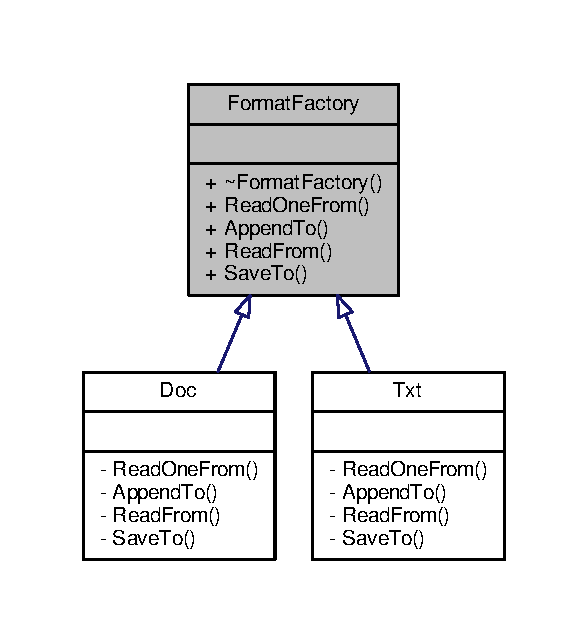
\includegraphics[width=282pt]{class_format_factory__inherit__graph}
\end{center}
\end{figure}


Граф связей класса Format\+Factory\+:\nopagebreak
\begin{figure}[H]
\begin{center}
\leavevmode
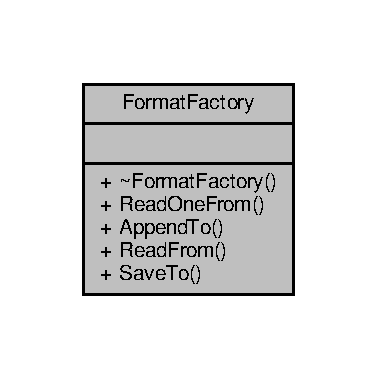
\includegraphics[width=181pt]{class_format_factory__coll__graph}
\end{center}
\end{figure}
\subsection*{Открытые члены}
\begin{DoxyCompactItemize}
\item 
virtual void \hyperlink{class_format_factory_a0002fa7430aefd926ac94c38155b146e}{Read\+One\+From} (bool \&flag, Q\+File \&file, \hyperlink{classgraph}{graph} \&FF)=0
\begin{DoxyCompactList}\small\item\em Функция чтения первой прямой из файла \end{DoxyCompactList}\item 
virtual void \hyperlink{class_format_factory_ae29ad79ca214f944962094487e668c8c}{Append\+To} (bool \&flag, Q\+File \&file, \hyperlink{classgraph}{graph} \&FF)=0
\begin{DoxyCompactList}\small\item\em Функция дописывания одной прямой в конец \end{DoxyCompactList}\item 
virtual void \hyperlink{class_format_factory_ad3136c43b27e86cf755106381081e67c}{Read\+From} (bool \&flag, Q\+File \&file, Q\+Vector$<$ \hyperlink{classgraph}{graph} $>$ \&FF)=0
\begin{DoxyCompactList}\small\item\em Функция чтения всех прямых из файла \end{DoxyCompactList}\item 
virtual void \hyperlink{class_format_factory_ac787363aa133a274ae674526dcc2b301}{Save\+To} (bool \&flag, Q\+File \&file, Q\+Vector$<$ \hyperlink{classgraph}{graph} $>$ \&FF)=0
\begin{DoxyCompactList}\small\item\em Функция сохранения всех прямых \end{DoxyCompactList}\end{DoxyCompactItemize}


\subsection{Подробное описание}
The \hyperlink{class_format_factory}{Format\+Factory} class. 

Абстрактный класс от которого производится наследование форматов 

См. определение в файле workwithfiles.\+h строка 19



\subsection{Методы}
\index{Format\+Factory@{Format\+Factory}!Append\+To@{Append\+To}}
\index{Append\+To@{Append\+To}!Format\+Factory@{Format\+Factory}}
\subsubsection[{\texorpdfstring{Append\+To(bool \&flag, Q\+File \&file, graph \&\+F\+F)=0}{AppendTo(bool &flag, QFile &file, graph &FF)=0}}]{\setlength{\rightskip}{0pt plus 5cm}virtual void Format\+Factory\+::\+Append\+To (
\begin{DoxyParamCaption}
\item[{bool \&}]{flag, }
\item[{Q\+File \&}]{file, }
\item[{{\bf graph} \&}]{FF}
\end{DoxyParamCaption}
)\hspace{0.3cm}{\ttfamily [pure virtual]}}\hypertarget{class_format_factory_ae29ad79ca214f944962094487e668c8c}{}\label{class_format_factory_ae29ad79ca214f944962094487e668c8c}


Функция дописывания одной прямой в конец 

Чисто виртуальная функция, уникальная для каждого класса наследника~\newline
см \hyperlink{class_txt_a4d23910d9b7f36e4f82fdf6045135378}{Txt\+::\+Append\+To()} и \hyperlink{class_doc_af5c9529b9108d9155b0d725f066b3d67}{Doc\+::\+Append\+To()} 
\begin{DoxyParams}{Аргументы}
{\em flag} & показатель записи 1 -\/ записано 0 -\/нет \\
\hline
{\em file} & ссылка на файл \\
\hline
{\em FF} & ссылка на нужную прямую \\
\hline
\end{DoxyParams}


Замещается в \hyperlink{class_doc_af5c9529b9108d9155b0d725f066b3d67}{Doc} и \hyperlink{class_txt_a4d23910d9b7f36e4f82fdf6045135378}{Txt}.

\index{Format\+Factory@{Format\+Factory}!Read\+From@{Read\+From}}
\index{Read\+From@{Read\+From}!Format\+Factory@{Format\+Factory}}
\subsubsection[{\texorpdfstring{Read\+From(bool \&flag, Q\+File \&file, Q\+Vector$<$ graph $>$ \&\+F\+F)=0}{ReadFrom(bool &flag, QFile &file, QVector< graph > &FF)=0}}]{\setlength{\rightskip}{0pt plus 5cm}virtual void Format\+Factory\+::\+Read\+From (
\begin{DoxyParamCaption}
\item[{bool \&}]{flag, }
\item[{Q\+File \&}]{file, }
\item[{Q\+Vector$<$ {\bf graph} $>$ \&}]{FF}
\end{DoxyParamCaption}
)\hspace{0.3cm}{\ttfamily [pure virtual]}}\hypertarget{class_format_factory_ad3136c43b27e86cf755106381081e67c}{}\label{class_format_factory_ad3136c43b27e86cf755106381081e67c}


Функция чтения всех прямых из файла 

Чисто виртуальная функция, уникальная для каждого класса наследника~\newline
см \hyperlink{class_txt_a2109a6bb72b2277dc5eb134a0f4f3257}{Txt\+::\+Read\+From()} и \hyperlink{class_doc_aa9359b8e110d9d26bcd25b68e1001743}{Doc\+::\+Read\+From()} 
\begin{DoxyParams}{Аргументы}
{\em flag} & удачно ли было проведено чтение 1 -\/ да 0 -\/нет \\
\hline
{\em file} & ссылка на файл \\
\hline
{\em FF} & промежуточный вектор с прямыми \\
\hline
\end{DoxyParams}


Замещается в \hyperlink{class_doc_aa9359b8e110d9d26bcd25b68e1001743}{Doc} и \hyperlink{class_txt_a2109a6bb72b2277dc5eb134a0f4f3257}{Txt}.



Используется в Main\+Window\+::on\+\_\+action\+Open\+\_\+file\+\_\+triggered().



Граф вызова функции\+:\nopagebreak
\begin{figure}[H]
\begin{center}
\leavevmode
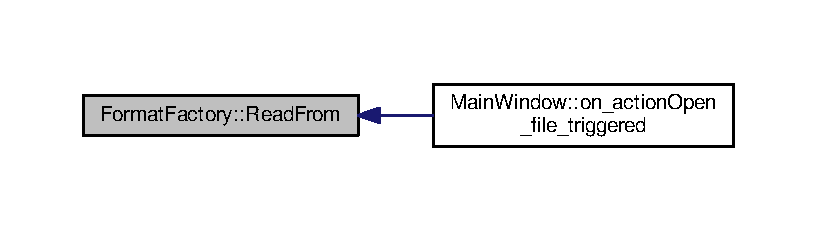
\includegraphics[width=350pt]{class_format_factory_ad3136c43b27e86cf755106381081e67c_icgraph}
\end{center}
\end{figure}


\index{Format\+Factory@{Format\+Factory}!Read\+One\+From@{Read\+One\+From}}
\index{Read\+One\+From@{Read\+One\+From}!Format\+Factory@{Format\+Factory}}
\subsubsection[{\texorpdfstring{Read\+One\+From(bool \&flag, Q\+File \&file, graph \&\+F\+F)=0}{ReadOneFrom(bool &flag, QFile &file, graph &FF)=0}}]{\setlength{\rightskip}{0pt plus 5cm}virtual void Format\+Factory\+::\+Read\+One\+From (
\begin{DoxyParamCaption}
\item[{bool \&}]{flag, }
\item[{Q\+File \&}]{file, }
\item[{{\bf graph} \&}]{FF}
\end{DoxyParamCaption}
)\hspace{0.3cm}{\ttfamily [pure virtual]}}\hypertarget{class_format_factory_a0002fa7430aefd926ac94c38155b146e}{}\label{class_format_factory_a0002fa7430aefd926ac94c38155b146e}


Функция чтения первой прямой из файла 

Чисто виртуальная функция, уникальная для каждого класса наследника~\newline
см \hyperlink{class_txt_a1fa6a42957c0e72314c7ba70eb3fab76}{Txt\+::\+Read\+One\+From()} и \hyperlink{class_doc_a3706c27d55dbb3fe7356a6b5dbb72b5c}{Doc\+::\+Read\+One\+From()} 
\begin{DoxyParams}{Аргументы}
{\em flag} & удачно ли было проведено чтение 1 -\/ да 0 -\/нет \\
\hline
{\em file} & ссылка на файл \\
\hline
{\em FF} & промежуточный вектор с прямыми \\
\hline
\end{DoxyParams}


Замещается в \hyperlink{class_doc_a3706c27d55dbb3fe7356a6b5dbb72b5c}{Doc} и \hyperlink{class_txt_a1fa6a42957c0e72314c7ba70eb3fab76}{Txt}.



Используется в Main\+Window\+::on\+\_\+action\+Open\+\_\+one\+\_\+curve\+\_\+triggered().



Граф вызова функции\+:\nopagebreak
\begin{figure}[H]
\begin{center}
\leavevmode
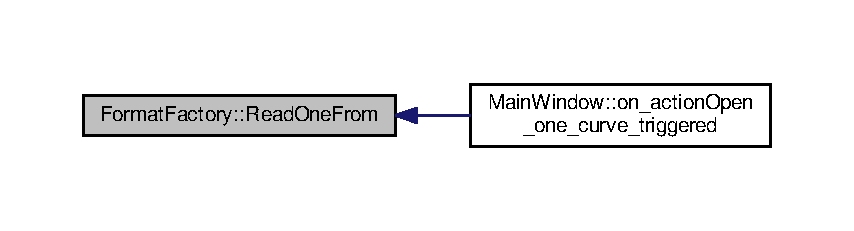
\includegraphics[width=350pt]{class_format_factory_a0002fa7430aefd926ac94c38155b146e_icgraph}
\end{center}
\end{figure}


\index{Format\+Factory@{Format\+Factory}!Save\+To@{Save\+To}}
\index{Save\+To@{Save\+To}!Format\+Factory@{Format\+Factory}}
\subsubsection[{\texorpdfstring{Save\+To(bool \&flag, Q\+File \&file, Q\+Vector$<$ graph $>$ \&\+F\+F)=0}{SaveTo(bool &flag, QFile &file, QVector< graph > &FF)=0}}]{\setlength{\rightskip}{0pt plus 5cm}virtual void Format\+Factory\+::\+Save\+To (
\begin{DoxyParamCaption}
\item[{bool \&}]{flag, }
\item[{Q\+File \&}]{file, }
\item[{Q\+Vector$<$ {\bf graph} $>$ \&}]{FF}
\end{DoxyParamCaption}
)\hspace{0.3cm}{\ttfamily [pure virtual]}}\hypertarget{class_format_factory_ac787363aa133a274ae674526dcc2b301}{}\label{class_format_factory_ac787363aa133a274ae674526dcc2b301}


Функция сохранения всех прямых 

Чисто виртуальная функция , уникальная для каждого класса наследника~\newline
см. \hyperlink{class_txt_abe4239811b140dd6fc5a439be6964aa0}{Txt\+::\+Save\+To()} и \hyperlink{class_doc_a00303c942160d3e6f69b38e387f12a03}{Doc\+::\+Save\+To()}~\newline

\begin{DoxyParams}{Аргументы}
{\em flag} & определяет удачна ли была запись 1 -\/ да 0 -\/ нет \\
\hline
{\em file} & ссылка на файл \\
\hline
{\em FF} & все прямые для записи \\
\hline
\end{DoxyParams}


Замещается в \hyperlink{class_doc_a00303c942160d3e6f69b38e387f12a03}{Doc} и \hyperlink{class_txt_abe4239811b140dd6fc5a439be6964aa0}{Txt}.



Используется в Main\+Window\+::on\+\_\+action\+Save\+\_\+\+File\+\_\+as\+\_\+triggered() и Main\+Window\+::on\+\_\+action\+Save\+\_\+\+File\+\_\+triggered().



Граф вызова функции\+:\nopagebreak
\begin{figure}[H]
\begin{center}
\leavevmode
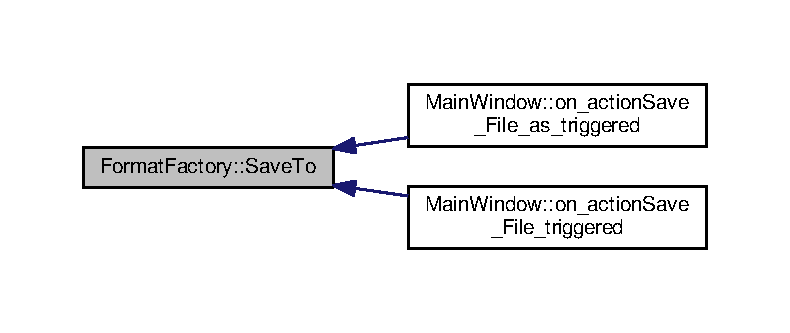
\includegraphics[width=350pt]{class_format_factory_ac787363aa133a274ae674526dcc2b301_icgraph}
\end{center}
\end{figure}




Объявления и описания членов класса находятся в файле\+:\begin{DoxyCompactItemize}
\item 
/home/silence/workplace/\+U\+I/c\+\_\+plus/\hyperlink{workwithfiles_8h}{workwithfiles.\+h}\end{DoxyCompactItemize}

\hypertarget{classgraph}{}\section{Класс graph}
\label{classgraph}\index{graph@{graph}}


The graph class.  




{\ttfamily \#include $<$mainwindow.\+h$>$}



Граф связей класса graph\+:\nopagebreak
\begin{figure}[H]
\begin{center}
\leavevmode
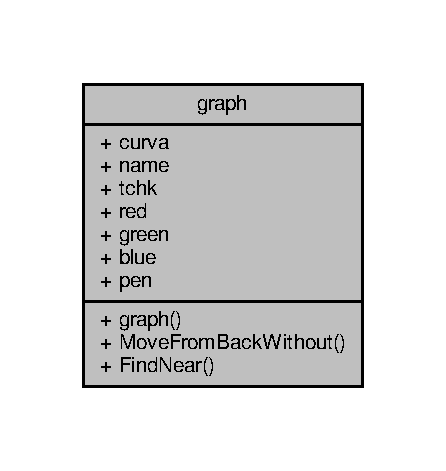
\includegraphics[width=214pt]{classgraph__coll__graph}
\end{center}
\end{figure}
\subsection*{Открытые члены}
\begin{DoxyCompactItemize}
\item 
\hyperlink{classgraph_a6aaa56b4528d2fdb8f0ecd97e04f6651}{graph} ()\hypertarget{classgraph_a6aaa56b4528d2fdb8f0ecd97e04f6651}{}\label{classgraph_a6aaa56b4528d2fdb8f0ecd97e04f6651}

\begin{DoxyCompactList}\small\item\em конструктор выделяет память под прямую Qwt\+Plot\+Curve. \end{DoxyCompactList}\item 
void \hyperlink{classgraph_af46434aacc2b15519b6a25943570ce05}{Move\+From\+Back\+Without} ()\hypertarget{classgraph_af46434aacc2b15519b6a25943570ce05}{}\label{classgraph_af46434aacc2b15519b6a25943570ce05}

\begin{DoxyCompactList}\small\item\em Функция, отвечающая за сортировку точек по координате x , с заменой точек с одинаковыми значениями новой \end{DoxyCompactList}\item 
int \hyperlink{classgraph_a69b8295dbfe6bcfab5050e3fdcc257f2}{Find\+Near} (double coordX, double coordY)
\begin{DoxyCompactList}\small\item\em Функция возвращающая индекс ближайшей точки к области клика \end{DoxyCompactList}\end{DoxyCompactItemize}
\subsection*{Открытые атрибуты}
\begin{DoxyCompactItemize}
\item 
Qwt\+Plot\+Curve $\ast$ \hyperlink{classgraph_abbfdc5f6022afe7be261bf927498e92e}{curva}\hypertarget{classgraph_abbfdc5f6022afe7be261bf927498e92e}{}\label{classgraph_abbfdc5f6022afe7be261bf927498e92e}

\begin{DoxyCompactList}\small\item\em Указатель на прямую , которая в итоге рисуется \end{DoxyCompactList}\item 
Q\+String \hyperlink{classgraph_abfbbdbd09b20d6ef147ee966b1325595}{name}\hypertarget{classgraph_abfbbdbd09b20d6ef147ee966b1325595}{}\label{classgraph_abfbbdbd09b20d6ef147ee966b1325595}

\begin{DoxyCompactList}\small\item\em Имя этой прямой \end{DoxyCompactList}\item 
Q\+Vector$<$ Q\+PointF $>$ \hyperlink{classgraph_afae7c6852c8de983693fb2fd108ed3c4}{tchk}\hypertarget{classgraph_afae7c6852c8de983693fb2fd108ed3c4}{}\label{classgraph_afae7c6852c8de983693fb2fd108ed3c4}

\begin{DoxyCompactList}\small\item\em Вектор, содержащий все точки прямой \end{DoxyCompactList}\item 
int \hyperlink{classgraph_aa3334acd551b2fc61901c2afdd4b2d8f}{red}\hypertarget{classgraph_aa3334acd551b2fc61901c2afdd4b2d8f}{}\label{classgraph_aa3334acd551b2fc61901c2afdd4b2d8f}

\begin{DoxyCompactList}\small\item\em Цвет прямой в формате R\+GB. \end{DoxyCompactList}\item 
int \hyperlink{classgraph_abb30b4156f98b6e0046f7192c389e4e4}{green}\hypertarget{classgraph_abb30b4156f98b6e0046f7192c389e4e4}{}\label{classgraph_abb30b4156f98b6e0046f7192c389e4e4}

\begin{DoxyCompactList}\small\item\em Цвет прямой в формате R\+GB. \end{DoxyCompactList}\item 
int \hyperlink{classgraph_a2007891f138555cc8be9ca822b9fa2db}{blue}\hypertarget{classgraph_a2007891f138555cc8be9ca822b9fa2db}{}\label{classgraph_a2007891f138555cc8be9ca822b9fa2db}

\begin{DoxyCompactList}\small\item\em Цвет прямой в формате R\+GB. \end{DoxyCompactList}\item 
double \hyperlink{classgraph_a237fa656ed0f8909b8eadd22aaeff422}{pen}\hypertarget{classgraph_a237fa656ed0f8909b8eadd22aaeff422}{}\label{classgraph_a237fa656ed0f8909b8eadd22aaeff422}

\begin{DoxyCompactList}\small\item\em Толщина прямой \end{DoxyCompactList}\end{DoxyCompactItemize}


\subsection{Подробное описание}
The graph class. 

Класс , содержащий все данные об одной прямой 

См. определение в файле mainwindow.\+h строка 64



\subsection{Методы}
\index{graph@{graph}!Find\+Near@{Find\+Near}}
\index{Find\+Near@{Find\+Near}!graph@{graph}}
\subsubsection[{\texorpdfstring{Find\+Near(double coord\+X, double coord\+Y)}{FindNear(double coordX, double coordY)}}]{\setlength{\rightskip}{0pt plus 5cm}int graph\+::\+Find\+Near (
\begin{DoxyParamCaption}
\item[{double}]{coordX, }
\item[{double}]{coordY}
\end{DoxyParamCaption}
)}\hypertarget{classgraph_a69b8295dbfe6bcfab5050e3fdcc257f2}{}\label{classgraph_a69b8295dbfe6bcfab5050e3fdcc257f2}


Функция возвращающая индекс ближайшей точки к области клика 

Индекс находится через наименьшую гипотенузу по теореме Пифагора 
\begin{DoxyParams}{Аргументы}
{\em coordX,coordY} & координты точки клика \\
\hline
\end{DoxyParams}
\begin{DoxyReturn}{Возвращает}
индекс ближайшей точки 
\end{DoxyReturn}


См. определение в файле mainwindow.\+cpp строка 347



Перекрестные ссылки tchk.


\begin{DoxyCode}
348 \{
349     \textcolor{keywordtype}{int} i,index=-1;
350     \textcolor{keywordtype}{double} mindlin=-1.0;
351     \textcolor{keywordtype}{int} bufdlin;
352     \textcolor{keywordflow}{if}(\hyperlink{classgraph_afae7c6852c8de983693fb2fd108ed3c4}{tchk}.size()>0)
353     \{
354         index=0;
355         mindlin=(\hyperlink{classgraph_afae7c6852c8de983693fb2fd108ed3c4}{tchk}[0].x()-coordX)*(\hyperlink{classgraph_afae7c6852c8de983693fb2fd108ed3c4}{tchk}[0].x()-coordX)+(\hyperlink{classgraph_afae7c6852c8de983693fb2fd108ed3c4}{tchk}[0].y()-coordY)*(
      \hyperlink{classgraph_afae7c6852c8de983693fb2fd108ed3c4}{tchk}[0].y()-coordY);
356     \}
357     \textcolor{keywordflow}{for}(i=1;i<\hyperlink{classgraph_afae7c6852c8de983693fb2fd108ed3c4}{tchk}.size();i++)
358     \{
359         bufdlin=(\hyperlink{classgraph_afae7c6852c8de983693fb2fd108ed3c4}{tchk}[i].x()-coordX)*(\hyperlink{classgraph_afae7c6852c8de983693fb2fd108ed3c4}{tchk}[i].x()-coordX)
360                 +(\hyperlink{classgraph_afae7c6852c8de983693fb2fd108ed3c4}{tchk}[i].y()-coordY)*(\hyperlink{classgraph_afae7c6852c8de983693fb2fd108ed3c4}{tchk}[i].y()-coordY);
361         \textcolor{keywordflow}{if}(bufdlin<mindlin)
362         \{
363             index=i;
364             mindlin=bufdlin;
365         \}
366     \}
367     \textcolor{keywordflow}{return} index;
368 \}
\end{DoxyCode}


Объявления и описания членов классов находятся в файлах\+:\begin{DoxyCompactItemize}
\item 
/home/silence/workplace/\+U\+I/c\+\_\+plus/\hyperlink{mainwindow_8h}{mainwindow.\+h}\item 
/home/silence/workplace/\+U\+I/c\+\_\+plus/mainwindow.\+cpp\end{DoxyCompactItemize}

\hypertarget{class_main_window}{}\section{Класс Main\+Window}
\label{class_main_window}\index{Main\+Window@{Main\+Window}}


The \hyperlink{class_main_window}{Main\+Window} class.  




{\ttfamily \#include $<$mainwindow.\+h$>$}



Граф наследования\+:Main\+Window\+:\nopagebreak
\begin{figure}[H]
\begin{center}
\leavevmode
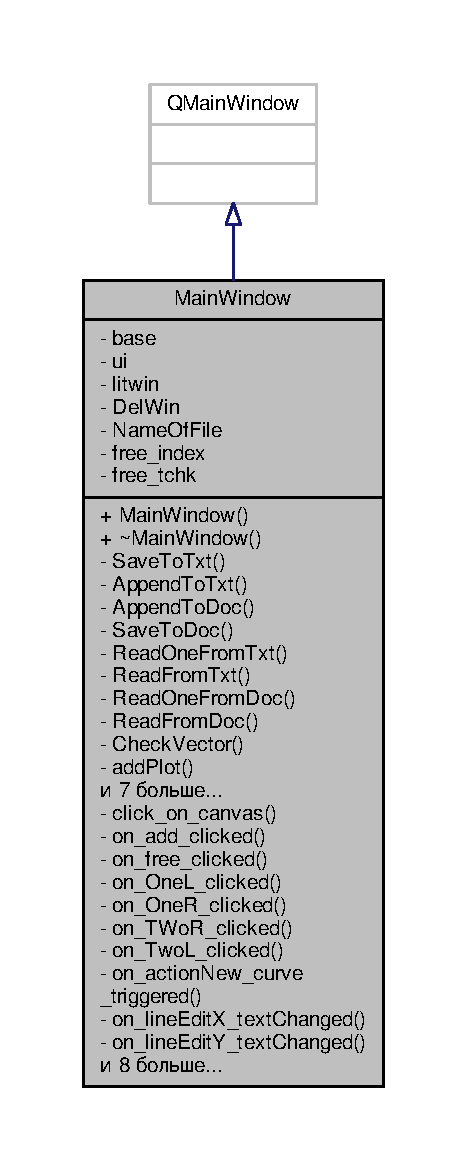
\includegraphics[height=550pt]{class_main_window__inherit__graph}
\end{center}
\end{figure}


Граф связей класса Main\+Window\+:\nopagebreak
\begin{figure}[H]
\begin{center}
\leavevmode
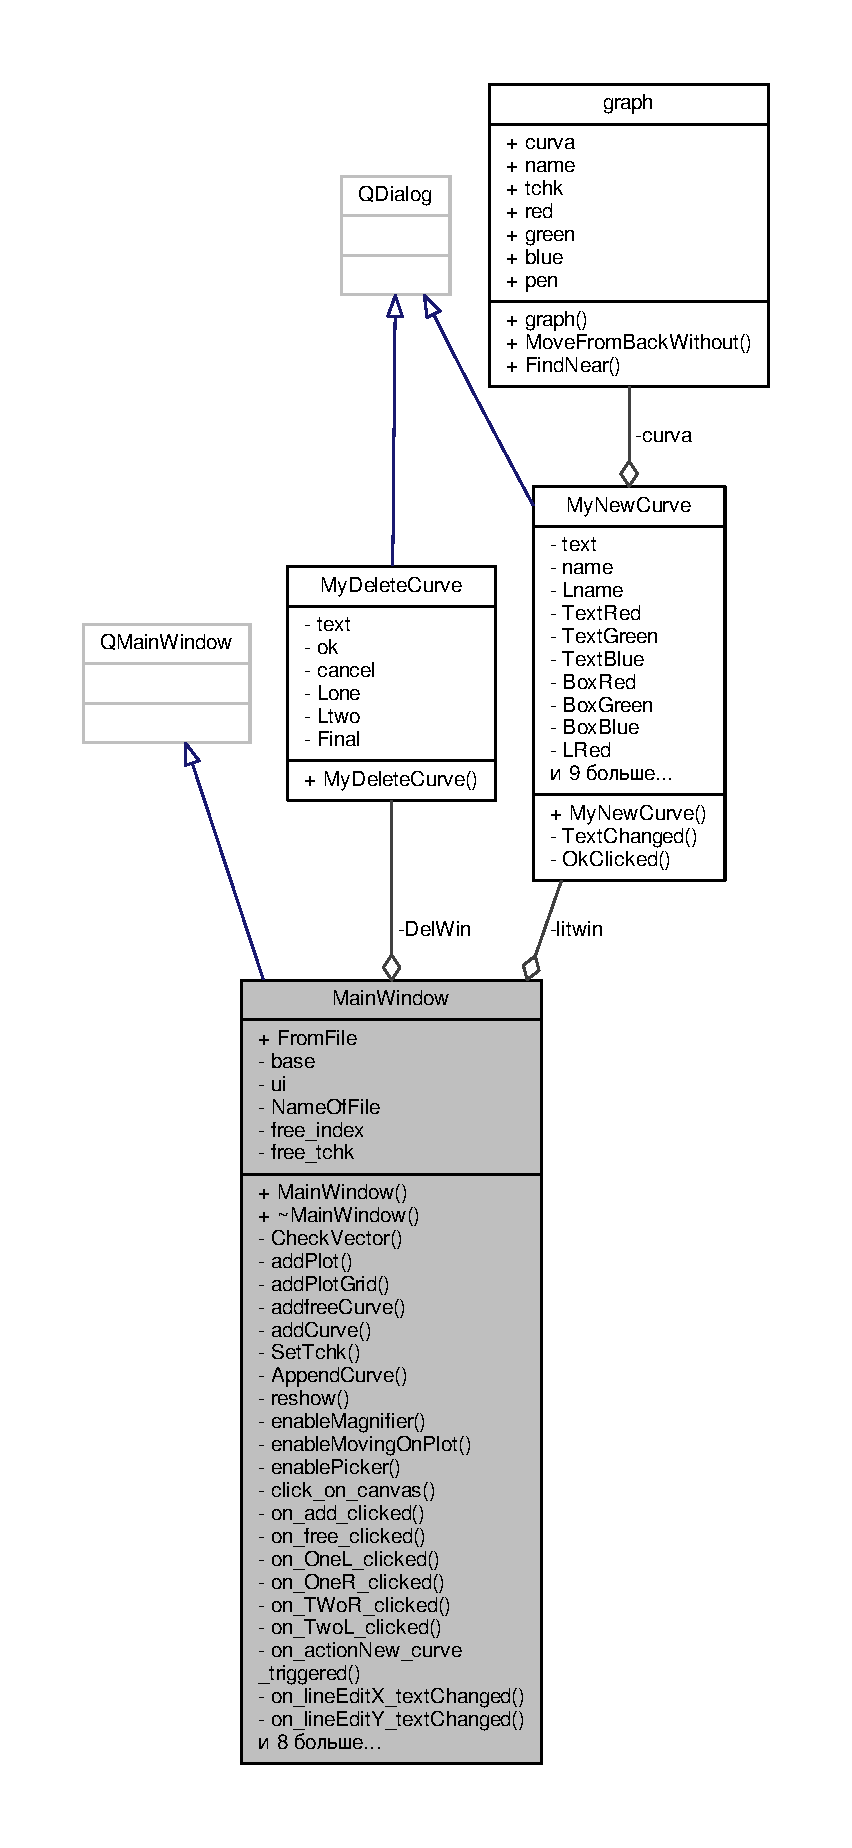
\includegraphics[height=550pt]{class_main_window__coll__graph}
\end{center}
\end{figure}
\subsection*{Открытые члены}
\begin{DoxyCompactItemize}
\item 
{\bfseries Main\+Window} (Q\+Widget $\ast$parent=0)\hypertarget{class_main_window_a8b244be8b7b7db1b08de2a2acb9409db}{}\label{class_main_window_a8b244be8b7b7db1b08de2a2acb9409db}

\end{DoxyCompactItemize}
\subsection*{Открытые атрибуты}
\begin{DoxyCompactItemize}
\item 
Q\+Vector$<$ \hyperlink{classgraph}{graph} $>$ {\bfseries From\+File}\hypertarget{class_main_window_a2c787b8ddb65b81709834176d660743c}{}\label{class_main_window_a2c787b8ddb65b81709834176d660743c}

\end{DoxyCompactItemize}
\subsection*{Закрытые слоты}
\begin{DoxyCompactItemize}
\item 
void \hyperlink{class_main_window_aa518cb3e5c52da2ccb6b886d6e09339d}{click\+\_\+on\+\_\+canvas} (const Q\+Point \&pos)\hypertarget{class_main_window_aa518cb3e5c52da2ccb6b886d6e09339d}{}\label{class_main_window_aa518cb3e5c52da2ccb6b886d6e09339d}

\begin{DoxyCompactList}\small\item\em Возвращает координаты клика по сетке \end{DoxyCompactList}\item 
void \hyperlink{class_main_window_ac5d7fe3c822551a9525b83fb6b3b99d3}{on\+\_\+add\+\_\+clicked} ()\hypertarget{class_main_window_ac5d7fe3c822551a9525b83fb6b3b99d3}{}\label{class_main_window_ac5d7fe3c822551a9525b83fb6b3b99d3}

\begin{DoxyCompactList}\small\item\em Добавить точку на активный график \end{DoxyCompactList}\item 
void \hyperlink{class_main_window_ad7f5879e59277f275c452d99d2d1e923}{on\+\_\+free\+\_\+clicked} ()\hypertarget{class_main_window_ad7f5879e59277f275c452d99d2d1e923}{}\label{class_main_window_ad7f5879e59277f275c452d99d2d1e923}

\begin{DoxyCompactList}\small\item\em Удаление точки с активного графика \end{DoxyCompactList}\item 
void \hyperlink{class_main_window_ac1cc49b084dceb4e44b973819b8bc9cc}{on\+\_\+\+One\+L\+\_\+clicked} ()\hypertarget{class_main_window_ac1cc49b084dceb4e44b973819b8bc9cc}{}\label{class_main_window_ac1cc49b084dceb4e44b973819b8bc9cc}

\begin{DoxyCompactList}\small\item\em Сдвиг точки для удаления влево по графику на 1. \end{DoxyCompactList}\item 
void \hyperlink{class_main_window_afa3f2fb370e2b3c9064880d9aa9a8d14}{on\+\_\+\+One\+R\+\_\+clicked} ()\hypertarget{class_main_window_afa3f2fb370e2b3c9064880d9aa9a8d14}{}\label{class_main_window_afa3f2fb370e2b3c9064880d9aa9a8d14}

\begin{DoxyCompactList}\small\item\em Сдвиг точки для удаления вправо по графику на 1. \end{DoxyCompactList}\item 
void \hyperlink{class_main_window_ac38bdf92edc1e6cbd07cced4497aa964}{on\+\_\+\+T\+Wo\+R\+\_\+clicked} ()\hypertarget{class_main_window_ac38bdf92edc1e6cbd07cced4497aa964}{}\label{class_main_window_ac38bdf92edc1e6cbd07cced4497aa964}

\begin{DoxyCompactList}\small\item\em Сдвиг на 10 точек вправо \end{DoxyCompactList}\item 
void \hyperlink{class_main_window_a3fd8329ca1b8ee5d2ac4da65ee5b6617}{on\+\_\+\+Two\+L\+\_\+clicked} ()\hypertarget{class_main_window_a3fd8329ca1b8ee5d2ac4da65ee5b6617}{}\label{class_main_window_a3fd8329ca1b8ee5d2ac4da65ee5b6617}

\begin{DoxyCompactList}\small\item\em Свдиг на 10 точек влево \end{DoxyCompactList}\item 
void \hyperlink{class_main_window_a39584a1d717e2430f7c8666071760335}{on\+\_\+action\+New\+\_\+curve\+\_\+triggered} ()\hypertarget{class_main_window_a39584a1d717e2430f7c8666071760335}{}\label{class_main_window_a39584a1d717e2430f7c8666071760335}

\begin{DoxyCompactList}\small\item\em Нажатие Edit-\/$>$New Curve. \end{DoxyCompactList}\item 
void \hyperlink{class_main_window_afa3811da5b85f09d356f9c417970fb5d}{on\+\_\+line\+Edit\+X\+\_\+text\+Changed} (const Q\+String \&arg1)\hypertarget{class_main_window_afa3811da5b85f09d356f9c417970fb5d}{}\label{class_main_window_afa3811da5b85f09d356f9c417970fb5d}

\begin{DoxyCompactList}\small\item\em Контроль непустого поля для добавления точки \end{DoxyCompactList}\item 
void \hyperlink{class_main_window_a5f00712967779082bc1e5099f139c0c4}{on\+\_\+line\+Edit\+Y\+\_\+text\+Changed} (const Q\+String \&arg1)\hypertarget{class_main_window_a5f00712967779082bc1e5099f139c0c4}{}\label{class_main_window_a5f00712967779082bc1e5099f139c0c4}

\begin{DoxyCompactList}\small\item\em Контроль непустого поля для добавления точки \end{DoxyCompactList}\item 
void \hyperlink{class_main_window_abe5494f1256abd53569e546236078ead}{on\+\_\+\+User\+Curve\+\_\+current\+Index\+Changed} (int index)\hypertarget{class_main_window_abe5494f1256abd53569e546236078ead}{}\label{class_main_window_abe5494f1256abd53569e546236078ead}

\begin{DoxyCompactList}\small\item\em Получения индекса активной прямой \end{DoxyCompactList}\item 
void \hyperlink{class_main_window_a6107fba5e2e27b6234ebcf703cf305b1}{on\+\_\+action\+Delete\+\_\+curve\+\_\+triggered} ()\hypertarget{class_main_window_a6107fba5e2e27b6234ebcf703cf305b1}{}\label{class_main_window_a6107fba5e2e27b6234ebcf703cf305b1}

\begin{DoxyCompactList}\small\item\em Нажатие Edit-\/$>$Delete Curve. \end{DoxyCompactList}\item 
void \hyperlink{class_main_window_ab4b13cfa6d7b65dfdea897e7e8425874}{on\+\_\+action\+Open\+\_\+file\+\_\+triggered} ()\hypertarget{class_main_window_ab4b13cfa6d7b65dfdea897e7e8425874}{}\label{class_main_window_ab4b13cfa6d7b65dfdea897e7e8425874}

\begin{DoxyCompactList}\small\item\em Нажатие Menu-\/$>$Open. \end{DoxyCompactList}\item 
void \hyperlink{class_main_window_ad0e823ebb5284bffb3eb92f95d6b0c79}{on\+\_\+action\+Save\+\_\+\+File\+\_\+as\+\_\+triggered} ()\hypertarget{class_main_window_ad0e823ebb5284bffb3eb92f95d6b0c79}{}\label{class_main_window_ad0e823ebb5284bffb3eb92f95d6b0c79}

\begin{DoxyCompactList}\small\item\em Нажатие Menu-\/$>$Save as. \end{DoxyCompactList}\item 
void \hyperlink{class_main_window_ab389ed5a61b95186643e6966ba965d5f}{on\+\_\+action\+Save\+\_\+\+File\+\_\+triggered} ()\hypertarget{class_main_window_ab389ed5a61b95186643e6966ba965d5f}{}\label{class_main_window_ab389ed5a61b95186643e6966ba965d5f}

\begin{DoxyCompactList}\small\item\em Нажатие Menu-\/$>$Save. \end{DoxyCompactList}\item 
void \hyperlink{class_main_window_a0c0436c2de50da0d7cf5b26242a694ad}{on\+\_\+action\+Open\+\_\+one\+\_\+curve\+\_\+triggered} ()\hypertarget{class_main_window_a0c0436c2de50da0d7cf5b26242a694ad}{}\label{class_main_window_a0c0436c2de50da0d7cf5b26242a694ad}

\begin{DoxyCompactList}\small\item\em Добавляет одну прямую из начала выбранного файла \end{DoxyCompactList}\item 
void \hyperlink{class_main_window_adb1ff161c75d24a3aa5d5aa71e3cbb91}{on\+\_\+action\+Save\+\_\+current\+\_\+curve\+\_\+triggered} ()\hypertarget{class_main_window_adb1ff161c75d24a3aa5d5aa71e3cbb91}{}\label{class_main_window_adb1ff161c75d24a3aa5d5aa71e3cbb91}

\begin{DoxyCompactList}\small\item\em Сохраняет одну прямую в конце текущего активного файла \end{DoxyCompactList}\item 
void \hyperlink{class_main_window_ad0e13c15f3efed36489c68de4bb6434f}{on\+\_\+action\+Save\+\_\+current\+\_\+curve\+\_\+as\+\_\+triggered} ()
\end{DoxyCompactItemize}
\subsection*{Закрытые члены}
\begin{DoxyCompactItemize}
\item 
void \hyperlink{class_main_window_a236bdec985319b80062b14e4e53bf2a0}{Check\+Vector} (bool \&okay)\hypertarget{class_main_window_a236bdec985319b80062b14e4e53bf2a0}{}\label{class_main_window_a236bdec985319b80062b14e4e53bf2a0}

\begin{DoxyCompactList}\small\item\em Проверяет есть ли существующие прямые при открытии файла.~\newline
 Если есть то предлагает их удалить и удаляет иначе открытие не произойдет \end{DoxyCompactList}\item 
void \hyperlink{class_main_window_a77cab55db6f0a5b74c9f7d3da47e006f}{add\+Plot} ()\hypertarget{class_main_window_a77cab55db6f0a5b74c9f7d3da47e006f}{}\label{class_main_window_a77cab55db6f0a5b74c9f7d3da47e006f}

\begin{DoxyCompactList}\small\item\em Добавляет график \end{DoxyCompactList}\item 
void \hyperlink{class_main_window_abb03c14d2a968e50a8d069b73f27efb0}{add\+Plot\+Grid} ()\hypertarget{class_main_window_abb03c14d2a968e50a8d069b73f27efb0}{}\label{class_main_window_abb03c14d2a968e50a8d069b73f27efb0}

\begin{DoxyCompactList}\small\item\em Добавляет сетку \end{DoxyCompactList}\item 
void \hyperlink{class_main_window_a3d6f33a054126933c27adefd9ea329e0}{addfree\+Curve} ()\hypertarget{class_main_window_a3d6f33a054126933c27adefd9ea329e0}{}\label{class_main_window_a3d6f33a054126933c27adefd9ea329e0}

\begin{DoxyCompactList}\small\item\em Добавление прямой из одной точки для подсветки активно \end{DoxyCompactList}\item 
void \hyperlink{class_main_window_aa5c0998b1192bfab3ff83b02c42b2c67}{add\+Curve} (\hyperlink{classgraph}{graph} \&buf)
\begin{DoxyCompactList}\small\item\em add\+Curve \end{DoxyCompactList}\item 
void \hyperlink{class_main_window_a167ea3c098e223361ff8d2300d71d6ae}{Set\+Tchk} ()\hypertarget{class_main_window_a167ea3c098e223361ff8d2300d71d6ae}{}\label{class_main_window_a167ea3c098e223361ff8d2300d71d6ae}

\begin{DoxyCompactList}\small\item\em Прикрепляет точки к графику после чтения из файла \end{DoxyCompactList}\item 
void \hyperlink{class_main_window_a28101a1eab9711200fbf177808d037eb}{Append\+Curve} (\hyperlink{classgraph}{graph} \&buf)\hypertarget{class_main_window_a28101a1eab9711200fbf177808d037eb}{}\label{class_main_window_a28101a1eab9711200fbf177808d037eb}

\begin{DoxyCompactList}\small\item\em Добавляет одну кривую вместе с точками \end{DoxyCompactList}\item 
void \hyperlink{class_main_window_a24985964bdf5f59467dcc99749e06bdd}{reshow} ()\hypertarget{class_main_window_a24985964bdf5f59467dcc99749e06bdd}{}\label{class_main_window_a24985964bdf5f59467dcc99749e06bdd}

\begin{DoxyCompactList}\small\item\em Используется для перезагрузки поля графиков, т.\+е. для отрисовки новых прямых \end{DoxyCompactList}\item 
void \hyperlink{class_main_window_afdb82afd72e8643eddf6f4c0266489e8}{enable\+Magnifier} ()\hypertarget{class_main_window_afdb82afd72e8643eddf6f4c0266489e8}{}\label{class_main_window_afdb82afd72e8643eddf6f4c0266489e8}

\begin{DoxyCompactList}\small\item\em Активация приближения по колесику мыши \end{DoxyCompactList}\item 
void \hyperlink{class_main_window_ad04c0aea2156c338a745b02ac456343b}{enable\+Moving\+On\+Plot} ()\hypertarget{class_main_window_ad04c0aea2156c338a745b02ac456343b}{}\label{class_main_window_ad04c0aea2156c338a745b02ac456343b}

\begin{DoxyCompactList}\small\item\em Активирует передвижение по сетке правой кнопкой мыши \end{DoxyCompactList}\item 
void \hyperlink{class_main_window_ac532634c85e6e35dfbd7c5d1c1520e62}{enable\+Picker} ()\hypertarget{class_main_window_ac532634c85e6e35dfbd7c5d1c1520e62}{}\label{class_main_window_ac532634c85e6e35dfbd7c5d1c1520e62}

\begin{DoxyCompactList}\small\item\em переводит координаты клика в полле ввода \end{DoxyCompactList}\end{DoxyCompactItemize}
\subsection*{Закрытые данные}
\begin{DoxyCompactItemize}
\item 
Q\+Vector$<$ \hyperlink{classgraph}{graph} $>$ \hyperlink{class_main_window_a3413d4508f4981518b1b8ebf3b29121e}{base}\hypertarget{class_main_window_a3413d4508f4981518b1b8ebf3b29121e}{}\label{class_main_window_a3413d4508f4981518b1b8ebf3b29121e}

\begin{DoxyCompactList}\small\item\em Содержит все прямые \end{DoxyCompactList}\item 
Ui\+::\+Main\+Window $\ast$ \hyperlink{class_main_window_a35466a70ed47252a0191168126a352a5}{ui}\hypertarget{class_main_window_a35466a70ed47252a0191168126a352a5}{}\label{class_main_window_a35466a70ed47252a0191168126a352a5}

\begin{DoxyCompactList}\small\item\em Указатель на форму главного окна \end{DoxyCompactList}\item 
\hyperlink{class_my_new_curve}{My\+New\+Curve} $\ast$ \hyperlink{class_main_window_a974a3a4a0c5646eca195d209856079dc}{litwin}\hypertarget{class_main_window_a974a3a4a0c5646eca195d209856079dc}{}\label{class_main_window_a974a3a4a0c5646eca195d209856079dc}

\begin{DoxyCompactList}\small\item\em Указатель на окно добавления новой прямой \end{DoxyCompactList}\item 
\hyperlink{class_my_delete_curve}{My\+Delete\+Curve} $\ast$ \hyperlink{class_main_window_a2f05d7f42a79bcda8f6e0fd216bf20d0}{Del\+Win}\hypertarget{class_main_window_a2f05d7f42a79bcda8f6e0fd216bf20d0}{}\label{class_main_window_a2f05d7f42a79bcda8f6e0fd216bf20d0}

\begin{DoxyCompactList}\small\item\em Указатель на окно удаления прямой \end{DoxyCompactList}\item 
Q\+String \hyperlink{class_main_window_a212db452b7d30710f776bc89a0a7e3ea}{Name\+Of\+File}\hypertarget{class_main_window_a212db452b7d30710f776bc89a0a7e3ea}{}\label{class_main_window_a212db452b7d30710f776bc89a0a7e3ea}

\begin{DoxyCompactList}\small\item\em Строка содержащая имя файла для функции Menu-\/$>$Save. \end{DoxyCompactList}\item 
int \hyperlink{class_main_window_a64477d24d552b3390b29fa2e8fe8d9ec}{free\+\_\+index}\hypertarget{class_main_window_a64477d24d552b3390b29fa2e8fe8d9ec}{}\label{class_main_window_a64477d24d552b3390b29fa2e8fe8d9ec}

\begin{DoxyCompactList}\small\item\em Индекс текущей точки для удаления \end{DoxyCompactList}\item 
Qwt\+Plot\+Curve $\ast$ \hyperlink{class_main_window_af61a9a165ff7529da09043c9538c5fe2}{free\+\_\+tchk}\hypertarget{class_main_window_af61a9a165ff7529da09043c9538c5fe2}{}\label{class_main_window_af61a9a165ff7529da09043c9538c5fe2}

\begin{DoxyCompactList}\small\item\em Прямая из одной точки, по сути подсвечивает активную точку для удаления \end{DoxyCompactList}\end{DoxyCompactItemize}


\subsection{Подробное описание}
The \hyperlink{class_main_window}{Main\+Window} class. 

Класс главного окна через которое происходит управление программой и в котором рисуются графики 

См. определение в файле mainwindow.\+h строка 101



\subsection{Методы}
\index{Main\+Window@{Main\+Window}!add\+Curve@{add\+Curve}}
\index{add\+Curve@{add\+Curve}!Main\+Window@{Main\+Window}}
\subsubsection[{\texorpdfstring{add\+Curve(graph \&buf)}{addCurve(graph &buf)}}]{\setlength{\rightskip}{0pt plus 5cm}void Main\+Window\+::add\+Curve (
\begin{DoxyParamCaption}
\item[{{\bf graph} \&}]{buf}
\end{DoxyParamCaption}
)\hspace{0.3cm}{\ttfamily [private]}}\hypertarget{class_main_window_aa5c0998b1192bfab3ff83b02c42b2c67}{}\label{class_main_window_aa5c0998b1192bfab3ff83b02c42b2c67}


add\+Curve 

Добавляет новою прямую в вектор из прямых 
\begin{DoxyParams}{Аргументы}
{\em buf} & ссылка по которой находится данные о прямой \\
\hline
\end{DoxyParams}


См. определение в файле mainwindow.\+cpp строка 65



Перекрестные ссылки base, graph\+::blue, graph\+::green, graph\+::name, graph\+::pen, graph\+::red и ui.



Используется в Append\+Curve(), on\+\_\+action\+New\+\_\+curve\+\_\+triggered() и Set\+Tchk().


\begin{DoxyCode}
66 \{
67     \textcolor{keywordtype}{int} index=\hyperlink{class_main_window_a3413d4508f4981518b1b8ebf3b29121e}{base}.size();\textcolor{comment}{//номер элемента в векторе base}
68     \hyperlink{class_main_window_a3413d4508f4981518b1b8ebf3b29121e}{base}.push\_back(\hyperlink{classgraph_a6aaa56b4528d2fdb8f0ecd97e04f6651}{graph}());
69     \hyperlink{class_main_window_a3413d4508f4981518b1b8ebf3b29121e}{base}[index].curva=\textcolor{keyword}{new} QwtPlotCurve;
70     \hyperlink{class_main_window_a3413d4508f4981518b1b8ebf3b29121e}{base}[index].name=buf.\hyperlink{classgraph_abfbbdbd09b20d6ef147ee966b1325595}{name};
71     \hyperlink{class_main_window_a3413d4508f4981518b1b8ebf3b29121e}{base}[index].red=buf.\hyperlink{classgraph_aa3334acd551b2fc61901c2afdd4b2d8f}{red};
72     \hyperlink{class_main_window_a3413d4508f4981518b1b8ebf3b29121e}{base}[index].green=buf.\hyperlink{classgraph_abb30b4156f98b6e0046f7192c389e4e4}{green};
73     \hyperlink{class_main_window_a3413d4508f4981518b1b8ebf3b29121e}{base}[index].blue=buf.\hyperlink{classgraph_a2007891f138555cc8be9ca822b9fa2db}{blue};
74     \hyperlink{class_main_window_a3413d4508f4981518b1b8ebf3b29121e}{base}[index].pen=buf.\hyperlink{classgraph_a237fa656ed0f8909b8eadd22aaeff422}{pen};
75     \hyperlink{class_main_window_a3413d4508f4981518b1b8ebf3b29121e}{base}[index].curva->setPen( QColor(buf.\hyperlink{classgraph_aa3334acd551b2fc61901c2afdd4b2d8f}{red},buf.\hyperlink{classgraph_abb30b4156f98b6e0046f7192c389e4e4}{green},buf.\hyperlink{classgraph_a2007891f138555cc8be9ca822b9fa2db}{blue}), buf.
      \hyperlink{classgraph_a237fa656ed0f8909b8eadd22aaeff422}{pen} );
76     \hyperlink{class_main_window_a3413d4508f4981518b1b8ebf3b29121e}{base}[index].curva->setRenderHint
77             ( QwtPlotItem::RenderAntialiased, \textcolor{keyword}{true} ); \textcolor{comment}{// сглаживание}
78     QwtSymbol *symbol = \textcolor{keyword}{new} QwtSymbol( QwtSymbol::Ellipse,
79     QBrush( Qt::white ), QPen( Qt::black ,3), QSize( 8, 8 ) );
80     \hyperlink{class_main_window_a3413d4508f4981518b1b8ebf3b29121e}{base}[index].curva->setSymbol( symbol );
81     \hyperlink{class_main_window_a3413d4508f4981518b1b8ebf3b29121e}{base}[index].curva->setTitle(buf.\hyperlink{classgraph_abfbbdbd09b20d6ef147ee966b1325595}{name});
82     \hyperlink{class_main_window_a35466a70ed47252a0191168126a352a5}{ui}->UserCurve->addItem(buf.\hyperlink{classgraph_abfbbdbd09b20d6ef147ee966b1325595}{name},index);
83     \hyperlink{class_main_window_a3413d4508f4981518b1b8ebf3b29121e}{base}[index].curva->attach( \hyperlink{class_main_window_a35466a70ed47252a0191168126a352a5}{ui}->Qwt\_Widget ); \textcolor{comment}{// отобразить кривую на графике}
84 
85 \}
\end{DoxyCode}


Граф вызова функции\+:\nopagebreak
\begin{figure}[H]
\begin{center}
\leavevmode
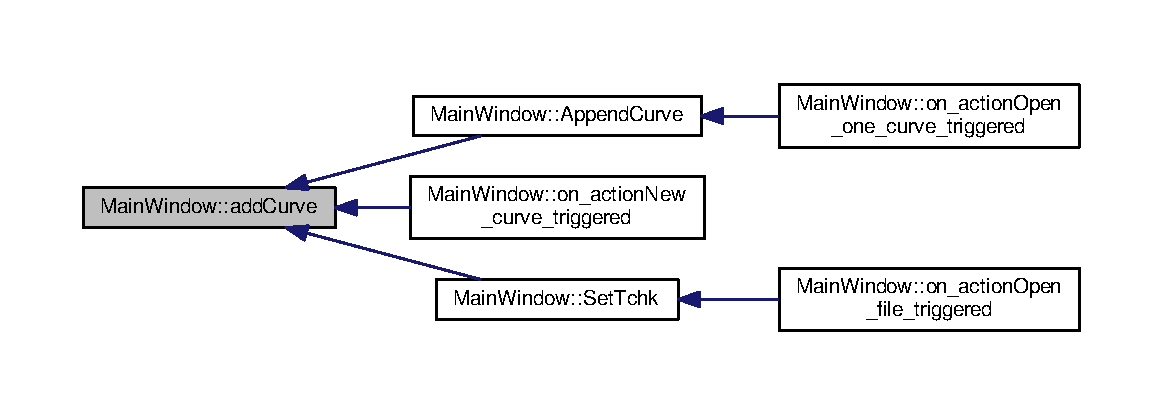
\includegraphics[width=350pt]{class_main_window_aa5c0998b1192bfab3ff83b02c42b2c67_icgraph}
\end{center}
\end{figure}


\index{Main\+Window@{Main\+Window}!on\+\_\+action\+Save\+\_\+current\+\_\+curve\+\_\+as\+\_\+triggered@{on\+\_\+action\+Save\+\_\+current\+\_\+curve\+\_\+as\+\_\+triggered}}
\index{on\+\_\+action\+Save\+\_\+current\+\_\+curve\+\_\+as\+\_\+triggered@{on\+\_\+action\+Save\+\_\+current\+\_\+curve\+\_\+as\+\_\+triggered}!Main\+Window@{Main\+Window}}
\subsubsection[{\texorpdfstring{on\+\_\+action\+Save\+\_\+current\+\_\+curve\+\_\+as\+\_\+triggered}{on_actionSave_current_curve_as_triggered}}]{\setlength{\rightskip}{0pt plus 5cm}void Main\+Window\+::on\+\_\+action\+Save\+\_\+current\+\_\+curve\+\_\+as\+\_\+triggered (
\begin{DoxyParamCaption}
{}
\end{DoxyParamCaption}
)\hspace{0.3cm}{\ttfamily [private]}, {\ttfamily [slot]}}\hypertarget{class_main_window_ad0e13c15f3efed36489c68de4bb6434f}{}\label{class_main_window_ad0e13c15f3efed36489c68de4bb6434f}
brief Сохраняет одну активную прямую в конец выбранного файла

\begin{DoxyWarning}{Предупреждения}
Не обращайте внимания на вопрос о замене файла, ничего не будет заменено. 
\end{DoxyWarning}


См. определение в файле mainwindow.\+cpp строка 630



Перекрестные ссылки Txt\+::\+Append\+To(), Doc\+::\+Append\+To(), base, Name\+Of\+File и ui.


\begin{DoxyCode}
631 \{
632     QString fileName = QFileDialog::getSaveFileName(\textcolor{keyword}{this}, tr(\textcolor{stringliteral}{"Save As"}), \textcolor{stringliteral}{"C://"},\textcolor{stringliteral}{".txt(*.txt);;.doc(*.doc)"})
      ;
633     \textcolor{keywordflow}{if} (fileName != \textcolor{stringliteral}{""})
634     \{
635 
636         \textcolor{keywordtype}{bool} flag=\textcolor{keyword}{false};
637         QFile file(fileName);
638         \textcolor{keywordflow}{if}(file.exists())
639             file.open(QIODevice::Append);
640         \textcolor{keywordflow}{if} (file.open(QIODevice::WriteOnly)||file.isOpen())
641         \{
642             \textcolor{keyword}{class }\hyperlink{classgraph}{graph} buf;
643             \hyperlink{class_format_factory}{FormatFactory}* WorkFile;
644             buf=\hyperlink{class_main_window_a3413d4508f4981518b1b8ebf3b29121e}{base}[\hyperlink{class_main_window_a35466a70ed47252a0191168126a352a5}{ui}->UserCurve->currentIndex()];
645             \textcolor{keywordflow}{if}(fileName[fileName.length()-1]==\textcolor{charliteral}{'t'})\textcolor{comment}{//определяем что txt}
646             \{
647                 WorkFile=\textcolor{keyword}{new} \hyperlink{class_txt}{Txt};
648                 WorkFile->\hyperlink{class_txt_a4d23910d9b7f36e4f82fdf6045135378}{AppendTo}(flag,file,buf);
649             \}
650             \textcolor{keywordflow}{if}(fileName[fileName.length()-1]==\textcolor{charliteral}{'c'})\textcolor{comment}{//А это док}
651             \{
652                 WorkFile=\textcolor{keyword}{new} \hyperlink{class_doc}{Doc};
653                 WorkFile->\hyperlink{class_doc_af5c9529b9108d9155b0d725f066b3d67}{AppendTo}(flag,file,buf);
654             \}
655             \textcolor{keywordflow}{if}(!flag)\textcolor{comment}{//Если запись не произошла}
656                 QMessageBox::critical(\textcolor{keyword}{this}, tr(\textcolor{stringliteral}{"Error"}), tr(\textcolor{stringliteral}{"Изменения не сохранены."})); \textcolor{comment}{//Типо если файл
       нельзя читать то ошибко.}
657             \textcolor{keywordflow}{else}\textcolor{comment}{//Записываем имя для повторного сохранения}
658             \{
659                 \hyperlink{class_main_window_a212db452b7d30710f776bc89a0a7e3ea}{NameOfFile}=fileName;
660                 QMessageBox::information(\textcolor{keyword}{this}, tr(\textcolor{stringliteral}{"Done"}),tr(\textcolor{stringliteral}{"Прямая %1 сохранена в %2"}).arg((
      \hyperlink{class_main_window_a3413d4508f4981518b1b8ebf3b29121e}{base}[\hyperlink{class_main_window_a35466a70ed47252a0191168126a352a5}{ui}->UserCurve->currentIndex()].name),\hyperlink{class_main_window_a212db452b7d30710f776bc89a0a7e3ea}{NameOfFile}));
661             \}
662             \textcolor{keyword}{delete} WorkFile;
663             file.close();
664         \}
665         \textcolor{keywordflow}{else}
666         \{
667             QMessageBox::critical(\textcolor{keyword}{this}, tr(\textcolor{stringliteral}{"Error"}), tr(\textcolor{stringliteral}{"Could not open file"})); \textcolor{comment}{//Нет прав на запись}
668             \textcolor{keywordflow}{return};
669         \}
670     \}
671     \textcolor{keywordflow}{else}
672         QMessageBox::critical(\textcolor{keyword}{this}, tr(\textcolor{stringliteral}{"Error"}), tr(\textcolor{stringliteral}{"Задан пустой путь до файла."})); \textcolor{comment}{//Типо если файл
       нельзя читать то ошибко.}
673 
674 \}
\end{DoxyCode}


Граф вызовов\+:\nopagebreak
\begin{figure}[H]
\begin{center}
\leavevmode
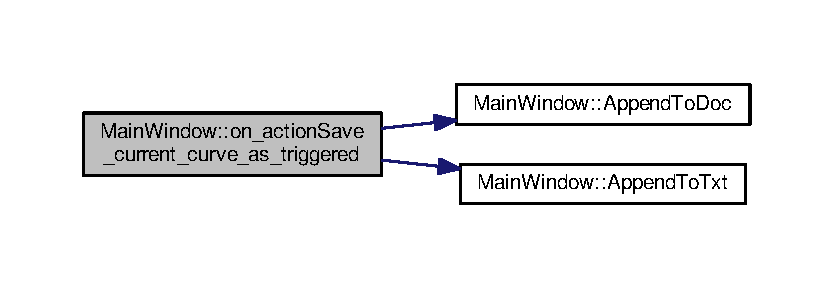
\includegraphics[width=344pt]{class_main_window_ad0e13c15f3efed36489c68de4bb6434f_cgraph}
\end{center}
\end{figure}




Объявления и описания членов классов находятся в файлах\+:\begin{DoxyCompactItemize}
\item 
/home/silence/workplace/\+U\+I/c\+\_\+plus/\hyperlink{mainwindow_8h}{mainwindow.\+h}\item 
/home/silence/workplace/\+U\+I/c\+\_\+plus/mainwindow.\+cpp\end{DoxyCompactItemize}

\hypertarget{class_my_delete_curve}{}\section{Класс My\+Delete\+Curve}
\label{class_my_delete_curve}\index{My\+Delete\+Curve@{My\+Delete\+Curve}}


The \hyperlink{class_my_delete_curve}{My\+Delete\+Curve} class.  




{\ttfamily \#include $<$mydialogcurve.\+h$>$}



Граф наследования\+:My\+Delete\+Curve\+:\nopagebreak
\begin{figure}[H]
\begin{center}
\leavevmode
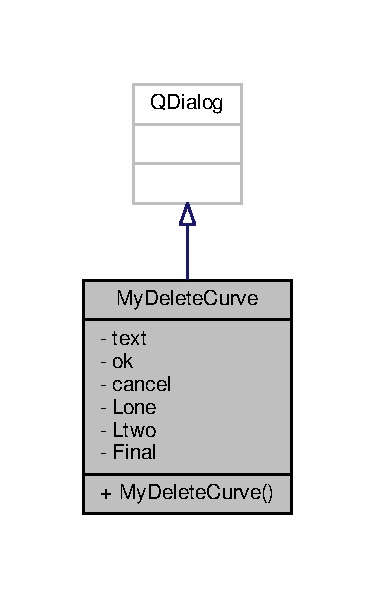
\includegraphics[width=180pt]{class_my_delete_curve__inherit__graph}
\end{center}
\end{figure}


Граф связей класса My\+Delete\+Curve\+:\nopagebreak
\begin{figure}[H]
\begin{center}
\leavevmode
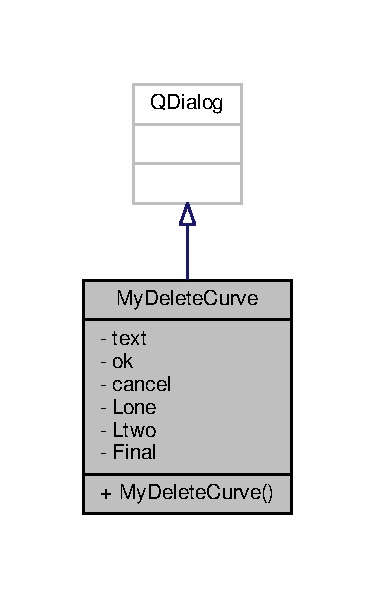
\includegraphics[width=180pt]{class_my_delete_curve__coll__graph}
\end{center}
\end{figure}
\subsection*{Открытые члены}
\begin{DoxyCompactItemize}
\item 
\hyperlink{class_my_delete_curve_af14574f71c84bf83931e5a9f3c124361}{My\+Delete\+Curve} (Q\+Widget $\ast$parent, Q\+String name)\hypertarget{class_my_delete_curve_af14574f71c84bf83931e5a9f3c124361}{}\label{class_my_delete_curve_af14574f71c84bf83931e5a9f3c124361}

\begin{DoxyCompactList}\small\item\em Получает имя строки для вывода \end{DoxyCompactList}\end{DoxyCompactItemize}
\subsection*{Закрытые данные}
\begin{DoxyCompactItemize}
\item 
Q\+Label $\ast$ {\bfseries text}\hypertarget{class_my_delete_curve_a6c229d6cb0a65941ea33d6c4553b827b}{}\label{class_my_delete_curve_a6c229d6cb0a65941ea33d6c4553b827b}

\item 
Q\+Push\+Button $\ast$ {\bfseries ok}\hypertarget{class_my_delete_curve_ad68069811a82e7652005a8bef1a4eea5}{}\label{class_my_delete_curve_ad68069811a82e7652005a8bef1a4eea5}

\item 
Q\+Push\+Button $\ast$ {\bfseries cancel}\hypertarget{class_my_delete_curve_a52214e1db933064bb5770ec3e55e982c}{}\label{class_my_delete_curve_a52214e1db933064bb5770ec3e55e982c}

\item 
Q\+H\+Box\+Layout $\ast$ {\bfseries Lone}\hypertarget{class_my_delete_curve_abd945d4ef22afe07394b8cd8711b538c}{}\label{class_my_delete_curve_abd945d4ef22afe07394b8cd8711b538c}

\item 
Q\+H\+Box\+Layout $\ast$ {\bfseries Ltwo}\hypertarget{class_my_delete_curve_a2c5bf4e6debf39d4a9823cac92d0c36a}{}\label{class_my_delete_curve_a2c5bf4e6debf39d4a9823cac92d0c36a}

\item 
Q\+V\+Box\+Layout $\ast$ {\bfseries Final}\hypertarget{class_my_delete_curve_ac6f2498b84a6196601fb2aa8c6465ff1}{}\label{class_my_delete_curve_ac6f2498b84a6196601fb2aa8c6465ff1}

\end{DoxyCompactItemize}


\subsection{Подробное описание}
The \hyperlink{class_my_delete_curve}{My\+Delete\+Curve} class. 

Класс окна удаления текущего активного графика. Весь смысл в том чтобы подтвердить удаление 

См. определение в файле mydialogcurve.\+h строка 65



Объявления и описания членов классов находятся в файлах\+:\begin{DoxyCompactItemize}
\item 
/home/silence/workplace/\+U\+I/c\+\_\+plus/\hyperlink{mydialogcurve_8h}{mydialogcurve.\+h}\item 
/home/silence/workplace/\+U\+I/c\+\_\+plus/mydialogcurve.\+cpp\end{DoxyCompactItemize}

\hypertarget{class_my_new_curve}{}\section{Класс My\+New\+Curve}
\label{class_my_new_curve}\index{My\+New\+Curve@{My\+New\+Curve}}


The \hyperlink{class_my_new_curve}{My\+New\+Curve} class.  




{\ttfamily \#include $<$mydialogcurve.\+h$>$}



Граф наследования\+:My\+New\+Curve\+:\nopagebreak
\begin{figure}[H]
\begin{center}
\leavevmode
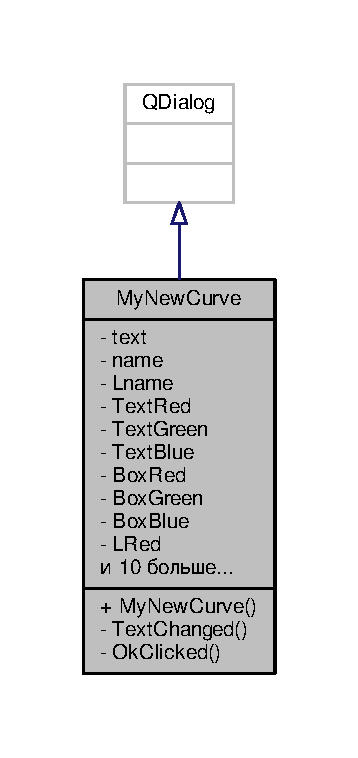
\includegraphics[width=172pt]{class_my_new_curve__inherit__graph}
\end{center}
\end{figure}


Граф связей класса My\+New\+Curve\+:\nopagebreak
\begin{figure}[H]
\begin{center}
\leavevmode
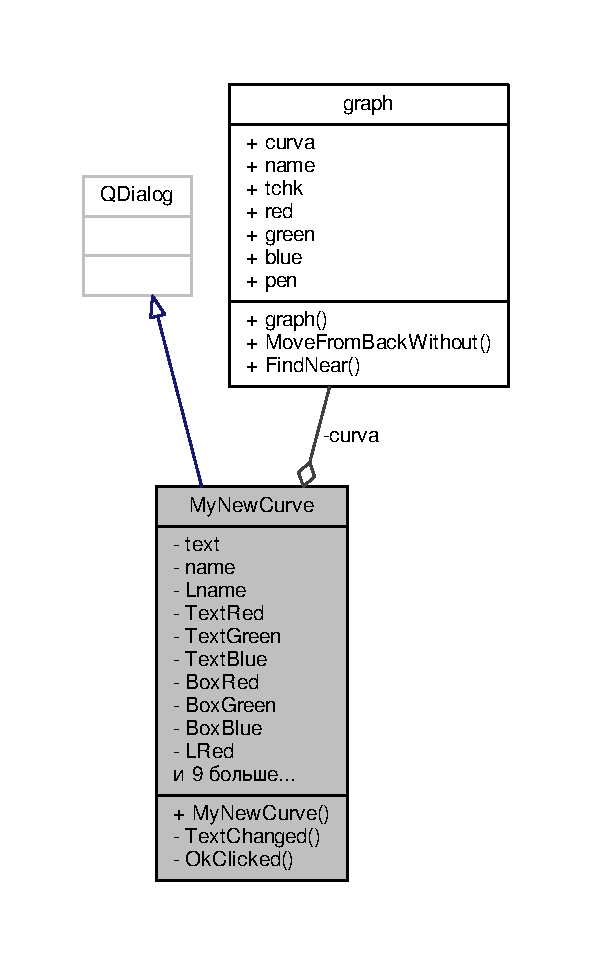
\includegraphics[width=284pt]{class_my_new_curve__coll__graph}
\end{center}
\end{figure}
\subsection*{Открытые члены}
\begin{DoxyCompactItemize}
\item 
\hyperlink{class_my_new_curve_a4bcbd4aa358bd6a043e9fc1ebffe7620}{My\+New\+Curve} (class \hyperlink{classgraph}{graph} \&nov, Q\+Widget $\ast$parent)\hypertarget{class_my_new_curve_a4bcbd4aa358bd6a043e9fc1ebffe7620}{}\label{class_my_new_curve_a4bcbd4aa358bd6a043e9fc1ebffe7620}

\begin{DoxyCompactList}\small\item\em При создании окно получает ссылку на класс прямой и заполняет его. \end{DoxyCompactList}\end{DoxyCompactItemize}
\subsection*{Закрытые слоты}
\begin{DoxyCompactItemize}
\item 
void \hyperlink{class_my_new_curve_ad2f0b68e3ac43c6046261ad41059edae}{Text\+Changed} (Q\+String str)\hypertarget{class_my_new_curve_ad2f0b68e3ac43c6046261ad41059edae}{}\label{class_my_new_curve_ad2f0b68e3ac43c6046261ad41059edae}

\begin{DoxyCompactList}\small\item\em Доступность кнопки ок \end{DoxyCompactList}\item 
void \hyperlink{class_my_new_curve_a220756368617b53ca4c70237ae018a08}{Ok\+Clicked} ()\hypertarget{class_my_new_curve_a220756368617b53ca4c70237ae018a08}{}\label{class_my_new_curve_a220756368617b53ca4c70237ae018a08}

\begin{DoxyCompactList}\small\item\em выход через accept , тоесть вернёт 1. \end{DoxyCompactList}\end{DoxyCompactItemize}
\subsection*{Закрытые данные}
\begin{DoxyCompactItemize}
\item 
Q\+Label $\ast$ {\bfseries text}\hypertarget{class_my_new_curve_afe5dcbf9eb1e8a508c62c47b1f1d8731}{}\label{class_my_new_curve_afe5dcbf9eb1e8a508c62c47b1f1d8731}

\item 
Q\+Line\+Edit $\ast$ {\bfseries name}\hypertarget{class_my_new_curve_a6b2024b3ff171df55727ddc1f14e650c}{}\label{class_my_new_curve_a6b2024b3ff171df55727ddc1f14e650c}

\item 
Q\+H\+Box\+Layout $\ast$ {\bfseries Lname}\hypertarget{class_my_new_curve_ae54f797a1a87a88451e123b6ec224138}{}\label{class_my_new_curve_ae54f797a1a87a88451e123b6ec224138}

\item 
Q\+Label $\ast$ {\bfseries Text\+Red}\hypertarget{class_my_new_curve_afcb0f8300093909c40d21b6d62cff50d}{}\label{class_my_new_curve_afcb0f8300093909c40d21b6d62cff50d}

\item 
Q\+Label $\ast$ {\bfseries Text\+Green}\hypertarget{class_my_new_curve_ae1c09f3bf69cfa8f90837107aeac3906}{}\label{class_my_new_curve_ae1c09f3bf69cfa8f90837107aeac3906}

\item 
Q\+Label $\ast$ {\bfseries Text\+Blue}\hypertarget{class_my_new_curve_aba072b80d92992948ba631f26106d0ba}{}\label{class_my_new_curve_aba072b80d92992948ba631f26106d0ba}

\item 
Q\+Spin\+Box $\ast$ {\bfseries Box\+Red}\hypertarget{class_my_new_curve_a37b211c94b00a2928c96f95157839deb}{}\label{class_my_new_curve_a37b211c94b00a2928c96f95157839deb}

\item 
Q\+Spin\+Box $\ast$ {\bfseries Box\+Green}\hypertarget{class_my_new_curve_abf842ae2344dc6ba03a57aa4f200b970}{}\label{class_my_new_curve_abf842ae2344dc6ba03a57aa4f200b970}

\item 
Q\+Spin\+Box $\ast$ {\bfseries Box\+Blue}\hypertarget{class_my_new_curve_adb5d040a4f9451af0d84e69761cc8905}{}\label{class_my_new_curve_adb5d040a4f9451af0d84e69761cc8905}

\item 
Q\+H\+Box\+Layout $\ast$ {\bfseries L\+Red}\hypertarget{class_my_new_curve_a5a9ee38f646cb061889c01e7da30df4b}{}\label{class_my_new_curve_a5a9ee38f646cb061889c01e7da30df4b}

\item 
Q\+H\+Box\+Layout $\ast$ {\bfseries L\+Green}\hypertarget{class_my_new_curve_a1e5abceba7257c0b9ecead84cfd9cc65}{}\label{class_my_new_curve_a1e5abceba7257c0b9ecead84cfd9cc65}

\item 
Q\+H\+Box\+Layout $\ast$ {\bfseries L\+Blue}\hypertarget{class_my_new_curve_a2d94abe7d24d0771c89b088eebd67746}{}\label{class_my_new_curve_a2d94abe7d24d0771c89b088eebd67746}

\item 
Q\+Label $\ast$ {\bfseries Text\+Thickness}\hypertarget{class_my_new_curve_acfe31b2fcdc46988b9dd1461d52e66b4}{}\label{class_my_new_curve_acfe31b2fcdc46988b9dd1461d52e66b4}

\item 
Q\+Double\+Spin\+Box $\ast$ {\bfseries Box\+Thickness}\hypertarget{class_my_new_curve_a3a82c01b232e4987874a140641bfae6a}{}\label{class_my_new_curve_a3a82c01b232e4987874a140641bfae6a}

\item 
Q\+H\+Box\+Layout $\ast$ {\bfseries L\+Thickness}\hypertarget{class_my_new_curve_ae945f7f28e50dfb0d5f8ec31d2d664db}{}\label{class_my_new_curve_ae945f7f28e50dfb0d5f8ec31d2d664db}

\item 
Q\+Push\+Button $\ast$ {\bfseries ok}\hypertarget{class_my_new_curve_aafb32d95590f926825a281f716399b60}{}\label{class_my_new_curve_aafb32d95590f926825a281f716399b60}

\item 
Q\+Push\+Button $\ast$ {\bfseries cancel}\hypertarget{class_my_new_curve_aaa33e47f0bec8d508bc21232b4f40c54}{}\label{class_my_new_curve_aaa33e47f0bec8d508bc21232b4f40c54}

\item 
Q\+H\+Box\+Layout $\ast$ {\bfseries L\+Push\+Button}\hypertarget{class_my_new_curve_aba3c9aa3c54ae37cbe0534850e50d127}{}\label{class_my_new_curve_aba3c9aa3c54ae37cbe0534850e50d127}

\item 
Q\+V\+Box\+Layout $\ast$ {\bfseries Final}\hypertarget{class_my_new_curve_a434922e9f8ef0c203cc5b092177b3d7f}{}\label{class_my_new_curve_a434922e9f8ef0c203cc5b092177b3d7f}

\item 
class \hyperlink{classgraph}{graph} $\ast$ {\bfseries curva}\hypertarget{class_my_new_curve_adc9b0d35a6dd14fbbb9dafb7d216d09e}{}\label{class_my_new_curve_adc9b0d35a6dd14fbbb9dafb7d216d09e}

\end{DoxyCompactItemize}


\subsection{Подробное описание}
The \hyperlink{class_my_new_curve}{My\+New\+Curve} class. 

Класс окна добавления нового графика.\+Вызывается при нажатии Edit-\/$>$New Curve внутрь окна заносится вся информация о прямой, после создания прямой в главном окне можно добавлять различные точки \begin{DoxyWarning}{Предупреждения}
Имя прямой не должно содержать только цифры. 
\end{DoxyWarning}


См. определение в файле mydialogcurve.\+h строка 31



Объявления и описания членов классов находятся в файлах\+:\begin{DoxyCompactItemize}
\item 
/home/silence/workplace/\+U\+I/c\+\_\+plus/\hyperlink{mydialogcurve_8h}{mydialogcurve.\+h}\item 
/home/silence/workplace/\+U\+I/c\+\_\+plus/mydialogcurve.\+cpp\end{DoxyCompactItemize}

\hypertarget{class_txt}{}\section{Класс Txt}
\label{class_txt}\index{Txt@{Txt}}


Класс для работы с .txt форматом  




{\ttfamily \#include $<$workwithfiles.\+h$>$}



Граф наследования\+:Txt\+:\nopagebreak
\begin{figure}[H]
\begin{center}
\leavevmode
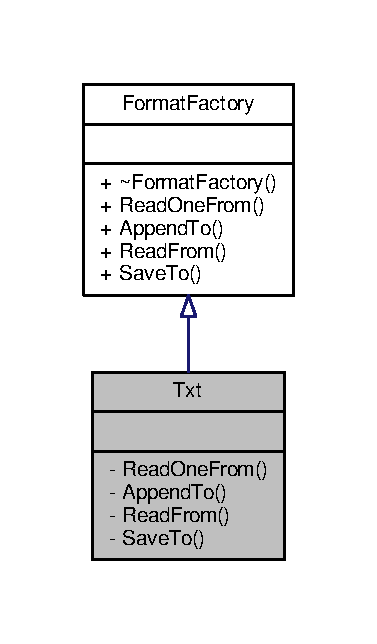
\includegraphics[width=181pt]{class_txt__inherit__graph}
\end{center}
\end{figure}


Граф связей класса Txt\+:\nopagebreak
\begin{figure}[H]
\begin{center}
\leavevmode
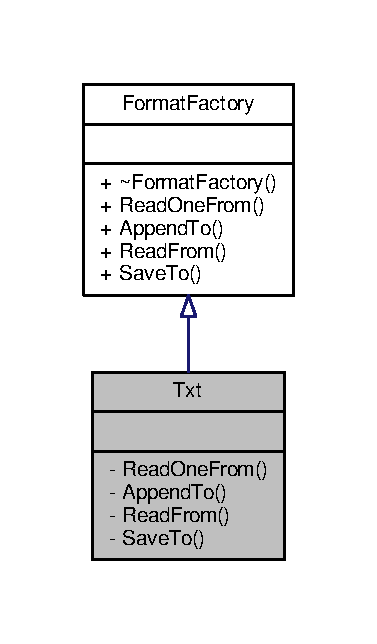
\includegraphics[width=181pt]{class_txt__coll__graph}
\end{center}
\end{figure}
\subsection*{Закрытые члены}
\begin{DoxyCompactItemize}
\item 
void \hyperlink{class_txt_a1fa6a42957c0e72314c7ba70eb3fab76}{Read\+One\+From} (bool \&flag, Q\+File \&file, \hyperlink{classgraph}{graph} \&FF)
\begin{DoxyCompactList}\small\item\em Читает одну прямую из .txt формата \end{DoxyCompactList}\item 
void \hyperlink{class_txt_a4d23910d9b7f36e4f82fdf6045135378}{Append\+To} (bool \&flag, Q\+File \&file, \hyperlink{classgraph}{graph} \&FF)
\begin{DoxyCompactList}\small\item\em Функция сохранения одной прямой в конец файла .txt. \end{DoxyCompactList}\item 
void \hyperlink{class_txt_a2109a6bb72b2277dc5eb134a0f4f3257}{Read\+From} (bool \&flag, Q\+File \&file, Q\+Vector$<$ \hyperlink{classgraph}{graph} $>$ \&FF)
\begin{DoxyCompactList}\small\item\em Читает все прямые из .txt формата \end{DoxyCompactList}\item 
void \hyperlink{class_txt_abe4239811b140dd6fc5a439be6964aa0}{Save\+To} (bool \&flag, Q\+File \&file, Q\+Vector$<$ \hyperlink{classgraph}{graph} $>$ \&FF)
\begin{DoxyCompactList}\small\item\em Функция сохранения в формат .txt. \end{DoxyCompactList}\end{DoxyCompactItemize}
\subsection*{Дополнительные унаследованные члены}


\subsection{Подробное описание}
Класс для работы с .txt форматом 

См. определение в файле workwithfiles.\+h строка 71



\subsection{Методы}
\index{Txt@{Txt}!Append\+To@{Append\+To}}
\index{Append\+To@{Append\+To}!Txt@{Txt}}
\subsubsection[{\texorpdfstring{Append\+To(bool \&flag, Q\+File \&file, graph \&\+F\+F)}{AppendTo(bool &flag, QFile &file, graph &FF)}}]{\setlength{\rightskip}{0pt plus 5cm}void Txt\+::\+Append\+To (
\begin{DoxyParamCaption}
\item[{bool \&}]{flag, }
\item[{Q\+File \&}]{file, }
\item[{{\bf graph} \&}]{FF}
\end{DoxyParamCaption}
)\hspace{0.3cm}{\ttfamily [private]}, {\ttfamily [virtual]}}\hypertarget{class_txt_a4d23910d9b7f36e4f82fdf6045135378}{}\label{class_txt_a4d23910d9b7f36e4f82fdf6045135378}


Функция сохранения одной прямой в конец файла .txt. 


\begin{DoxyParams}{Аргументы}
{\em flag} & показатель 1 -\/ записано 0 -\/нет \\
\hline
{\em file} & ссылка на файл \\
\hline
{\em FF} & ссылка на нужную прямую \\
\hline
\end{DoxyParams}


Замещает \hyperlink{class_format_factory_ae29ad79ca214f944962094487e668c8c}{Format\+Factory}.



См. определение в файле workwithfiles.\+cpp строка 17



Перекрестные ссылки graph\+::blue, graph\+::green, graph\+::name, graph\+::pen, graph\+::red и graph\+::tchk.



Используется в Main\+Window\+::on\+\_\+action\+Save\+\_\+current\+\_\+curve\+\_\+as\+\_\+triggered() и Main\+Window\+::on\+\_\+action\+Save\+\_\+current\+\_\+curve\+\_\+triggered().


\begin{DoxyCode}
18 \{
19 
20     QTextStream out(&file);
21     out << FF.\hyperlink{classgraph_abfbbdbd09b20d6ef147ee966b1325595}{name} << \textcolor{stringliteral}{"\(\backslash\)n"} << FF.\hyperlink{classgraph_aa3334acd551b2fc61901c2afdd4b2d8f}{red} << \textcolor{stringliteral}{"\(\backslash\)n"} << FF.\hyperlink{classgraph_abb30b4156f98b6e0046f7192c389e4e4}{green} << \textcolor{stringliteral}{"\(\backslash\)n"} << FF.
      \hyperlink{classgraph_a2007891f138555cc8be9ca822b9fa2db}{blue} << \textcolor{stringliteral}{"\(\backslash\)n"} << FF.\hyperlink{classgraph_a237fa656ed0f8909b8eadd22aaeff422}{pen} << \textcolor{stringliteral}{"\(\backslash\)n"};
22     \textcolor{keywordflow}{for}(\textcolor{keywordtype}{int} j=0; j<FF.\hyperlink{classgraph_afae7c6852c8de983693fb2fd108ed3c4}{tchk}.size();j++)
23         out<<FF.\hyperlink{classgraph_afae7c6852c8de983693fb2fd108ed3c4}{tchk}[j].x()<<\textcolor{stringliteral}{"\(\backslash\)n"}<<FF.\hyperlink{classgraph_afae7c6852c8de983693fb2fd108ed3c4}{tchk}[j].y()<<\textcolor{stringliteral}{"\(\backslash\)n"};
24     flag=\textcolor{keyword}{true};
25 \}
\end{DoxyCode}


Граф вызова функции\+:\nopagebreak
\begin{figure}[H]
\begin{center}
\leavevmode
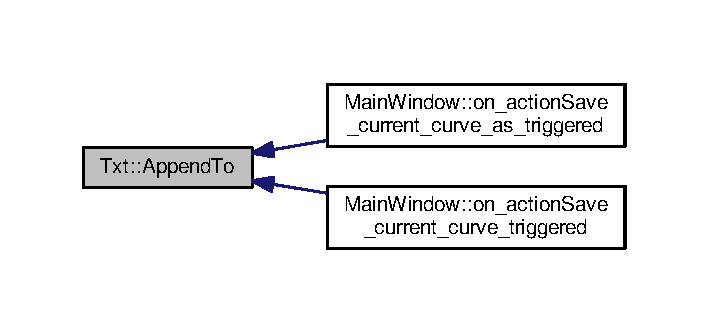
\includegraphics[width=340pt]{class_txt_a4d23910d9b7f36e4f82fdf6045135378_icgraph}
\end{center}
\end{figure}


\index{Txt@{Txt}!Read\+From@{Read\+From}}
\index{Read\+From@{Read\+From}!Txt@{Txt}}
\subsubsection[{\texorpdfstring{Read\+From(bool \&flag, Q\+File \&file, Q\+Vector$<$ graph $>$ \&\+F\+F)}{ReadFrom(bool &flag, QFile &file, QVector< graph > &FF)}}]{\setlength{\rightskip}{0pt plus 5cm}void Txt\+::\+Read\+From (
\begin{DoxyParamCaption}
\item[{bool \&}]{flag, }
\item[{Q\+File \&}]{file, }
\item[{Q\+Vector$<$ {\bf graph} $>$ \&}]{FF}
\end{DoxyParamCaption}
)\hspace{0.3cm}{\ttfamily [private]}, {\ttfamily [virtual]}}\hypertarget{class_txt_a2109a6bb72b2277dc5eb134a0f4f3257}{}\label{class_txt_a2109a6bb72b2277dc5eb134a0f4f3257}


Читает все прямые из .txt формата 

\begin{DoxyWarning}{Предупреждения}
Прямые должны быть оформлены соответственно.~\newline
смотрите \hyperlink{class_txt_abe4239811b140dd6fc5a439be6964aa0}{Txt\+::\+Save\+To()}; 
\end{DoxyWarning}

\begin{DoxyParams}{Аргументы}
{\em flag} & удачно ли было проведено чтение 1 -\/ да 0 -\/нет \\
\hline
{\em file} & ссылка на файл \\
\hline
{\em FF} & промежуточный вектор с прямыми \\
\hline
\end{DoxyParams}


Замещает \hyperlink{class_format_factory_ad3136c43b27e86cf755106381081e67c}{Format\+Factory}.



См. определение в файле workwithfiles.\+cpp строка 26



Перекрестные ссылки graph\+::blue, graph\+::green, graph\+::name, graph\+::pen и graph\+::red.


\begin{DoxyCode}
27 \{
28     \textcolor{keywordtype}{bool} ok;
29     QTextStream in(&file);
30     \textcolor{keyword}{class }\hyperlink{classgraph}{graph} nov;
31     \textcolor{keywordtype}{int} i=-1;
32     \textcolor{keywordflow}{while}(1)
33     \{
34         QString buf;
35         buf=in.readLine();
36         \textcolor{keywordflow}{if}(buf.isEmpty())
37         \{
38 
39             flag=\textcolor{keyword}{true};
40             \textcolor{keywordflow}{break};
41         \}
42         buf.toDouble(&ok);
43         \textcolor{keywordflow}{if}(!ok)
44         \{
45             nov.\hyperlink{classgraph_abfbbdbd09b20d6ef147ee966b1325595}{name}=buf;
46             buf=in.readLine();
47             nov.red=buf.toInt();
48             buf=in.readLine();
49             nov.green=buf.toInt();
50             buf=in.readLine();
51             nov.blue=buf.toInt();
52             buf=in.readLine();
53             nov.pen=buf.toDouble();
54             \textcolor{comment}{//addCurve(nov);}
55             FF.push\_back(nov);
56             i++;
57         \}
58         \textcolor{keywordflow}{else}
59         \{
60             QString bufy;
61             bufy=in.readLine();
62             FF[i].tchk.push\_back(QPointF(buf.toDouble(),bufy.toDouble()));
63         \}
64 
65     \}
66 \}
\end{DoxyCode}
\index{Txt@{Txt}!Read\+One\+From@{Read\+One\+From}}
\index{Read\+One\+From@{Read\+One\+From}!Txt@{Txt}}
\subsubsection[{\texorpdfstring{Read\+One\+From(bool \&flag, Q\+File \&file, graph \&\+F\+F)}{ReadOneFrom(bool &flag, QFile &file, graph &FF)}}]{\setlength{\rightskip}{0pt plus 5cm}void Txt\+::\+Read\+One\+From (
\begin{DoxyParamCaption}
\item[{bool \&}]{flag, }
\item[{Q\+File \&}]{file, }
\item[{{\bf graph} \&}]{FF}
\end{DoxyParamCaption}
)\hspace{0.3cm}{\ttfamily [private]}, {\ttfamily [virtual]}}\hypertarget{class_txt_a1fa6a42957c0e72314c7ba70eb3fab76}{}\label{class_txt_a1fa6a42957c0e72314c7ba70eb3fab76}


Читает одну прямую из .txt формата 

\begin{DoxyWarning}{Предупреждения}
Прямые должны быть оформлены соответственно.~\newline
смотрите \hyperlink{class_txt_abe4239811b140dd6fc5a439be6964aa0}{Txt\+::\+Save\+To()}; 
\end{DoxyWarning}

\begin{DoxyParams}{Аргументы}
{\em flag} & удачно ли было проведено чтение 1 -\/ да 0 -\/нет \\
\hline
{\em file} & ссылка на файл \\
\hline
{\em FF} & промежуточный вектор с прямыми \\
\hline
\end{DoxyParams}


Замещает \hyperlink{class_format_factory_a0002fa7430aefd926ac94c38155b146e}{Format\+Factory}.



См. определение в файле workwithfiles.\+cpp строка 67



Перекрестные ссылки graph\+::blue, graph\+::green, graph\+::name, graph\+::pen, graph\+::red и graph\+::tchk.


\begin{DoxyCode}
68 \{
69     QTextStream in(&file);
70     \textcolor{comment}{//class graph nov;}
71     QString buf;
72     buf=in.readLine();
73     FF.\hyperlink{classgraph_abfbbdbd09b20d6ef147ee966b1325595}{name}=buf;
74     buf=in.readLine();
75     FF.\hyperlink{classgraph_aa3334acd551b2fc61901c2afdd4b2d8f}{red}=buf.toInt();
76     buf=in.readLine();
77     FF.\hyperlink{classgraph_abb30b4156f98b6e0046f7192c389e4e4}{green}=buf.toInt();
78     buf=in.readLine();
79     FF.\hyperlink{classgraph_a2007891f138555cc8be9ca822b9fa2db}{blue}=buf.toInt();
80     buf=in.readLine();
81     FF.\hyperlink{classgraph_a237fa656ed0f8909b8eadd22aaeff422}{pen}=buf.toDouble();
82     \textcolor{comment}{//addCurve(FF);}
83     \textcolor{keywordtype}{bool} ok;
84     \textcolor{keywordflow}{while}(1)
85     \{
86         buf=in.readLine();
87         buf.toDouble(&ok);
88         \textcolor{keywordflow}{if}(buf.isEmpty() || ok==\textcolor{keyword}{false})
89             \textcolor{keywordflow}{break};
90         QString bufy;
91         bufy=in.readLine();
92         FF.\hyperlink{classgraph_afae7c6852c8de983693fb2fd108ed3c4}{tchk}.push\_back(QPointF(buf.toDouble(),bufy.toDouble()));
93     \}
94 
95     flag=\textcolor{keyword}{true};
96 \}
\end{DoxyCode}
\index{Txt@{Txt}!Save\+To@{Save\+To}}
\index{Save\+To@{Save\+To}!Txt@{Txt}}
\subsubsection[{\texorpdfstring{Save\+To(bool \&flag, Q\+File \&file, Q\+Vector$<$ graph $>$ \&\+F\+F)}{SaveTo(bool &flag, QFile &file, QVector< graph > &FF)}}]{\setlength{\rightskip}{0pt plus 5cm}void Txt\+::\+Save\+To (
\begin{DoxyParamCaption}
\item[{bool \&}]{flag, }
\item[{Q\+File \&}]{file, }
\item[{Q\+Vector$<$ {\bf graph} $>$ \&}]{FF}
\end{DoxyParamCaption}
)\hspace{0.3cm}{\ttfamily [private]}, {\ttfamily [virtual]}}\hypertarget{class_txt_abe4239811b140dd6fc5a439be6964aa0}{}\label{class_txt_abe4239811b140dd6fc5a439be6964aa0}


Функция сохранения в формат .txt. 

\begin{DoxyWarning}{Предупреждения}
установлен определнный порядок расположения данных,необходимый для чтения данных , а именно \+: ~\newline
Имя прямой~\newline
Красный цвет~\newline
Зелеый цвет~\newline
Синий цвет~\newline
Толщина~\newline
Координата по x~\newline
Координата по y~\newline

\end{DoxyWarning}

\begin{DoxyParams}{Аргументы}
{\em flag} & определяет удачна ли была запись 1 -\/ да 0 -\/ нет \\
\hline
{\em file} & ссылка на файл \\
\hline
{\em FF} & все прямые для записи \\
\hline
\end{DoxyParams}


Замещает \hyperlink{class_format_factory_ac787363aa133a274ae674526dcc2b301}{Format\+Factory}.



См. определение в файле workwithfiles.\+cpp строка 5


\begin{DoxyCode}
6 \{
7     QTextStream out(&file);
8     \textcolor{keywordflow}{for}(\textcolor{keywordtype}{int} i=0; i<FF.size(); i++)
9     \{
10         out << FF[i].name << \textcolor{stringliteral}{"\(\backslash\)n"} << FF[i].red << \textcolor{stringliteral}{"\(\backslash\)n"} << FF[i].green << \textcolor{stringliteral}{"\(\backslash\)n"} << FF[i].blue << \textcolor{stringliteral}{"\(\backslash\)n"} << FF[i
      ].pen << \textcolor{stringliteral}{"\(\backslash\)n"};
11         \textcolor{keywordflow}{for}(\textcolor{keywordtype}{int} j=0; j<FF[i].tchk.size();j++)
12             out<<FF[i].\hyperlink{classgraph_afae7c6852c8de983693fb2fd108ed3c4}{tchk}[j].x()<<\textcolor{stringliteral}{"\(\backslash\)n"}<<FF[i].tchk[j].y()<<\textcolor{stringliteral}{"\(\backslash\)n"};
13     \}
14     flag=\textcolor{keyword}{true};
15 
16 \}
\end{DoxyCode}


Объявления и описания членов классов находятся в файлах\+:\begin{DoxyCompactItemize}
\item 
/home/silence/workplace/\+U\+I/c\+\_\+plus/\hyperlink{workwithfiles_8h}{workwithfiles.\+h}\item 
/home/silence/workplace/\+U\+I/c\+\_\+plus/workwithfiles.\+cpp\end{DoxyCompactItemize}

\chapter{Файлы}
\hypertarget{mainwindow_8h}{}\section{Файл /home/silence/workplace/\+U\+I/c\+\_\+plus/mainwindow.h}
\label{mainwindow_8h}\index{/home/silence/workplace/\+U\+I/c\+\_\+plus/mainwindow.\+h@{/home/silence/workplace/\+U\+I/c\+\_\+plus/mainwindow.\+h}}


Загловочный файл содержащий класс прямой и главное окно , в котором и рисуются прямые  


{\ttfamily \#include \char`\"{}mydialogcurve.\+h\char`\"{}}\\*
{\ttfamily \#include $<$Q\+Main\+Window$>$}\\*
{\ttfamily \#include $<$qwt\+\_\+plot.\+h$>$}\\*
{\ttfamily \#include $<$qwt\+\_\+plot\+\_\+grid.\+h$>$}\\*
{\ttfamily \#include $<$qwt\+\_\+legend.\+h$>$}\\*
{\ttfamily \#include $<$qwt\+\_\+plot\+\_\+curve.\+h$>$}\\*
{\ttfamily \#include $<$qwt\+\_\+symbol.\+h$>$}\\*
{\ttfamily \#include $<$qwt\+\_\+plot\+\_\+magnifier.\+h$>$}\\*
{\ttfamily \#include $<$qwt\+\_\+plot\+\_\+panner.\+h$>$}\\*
{\ttfamily \#include $<$qwt\+\_\+plot\+\_\+picker.\+h$>$}\\*
{\ttfamily \#include $<$qwt\+\_\+picker\+\_\+machine.\+h$>$}\\*
{\ttfamily \#include $<$Q\+Vector$>$}\\*
{\ttfamily \#include $<$Q\+Message\+Box$>$}\\*
{\ttfamily \#include $<$Q\+File\+Dialog$>$}\\*
{\ttfamily \#include $<$Q\+File$>$}\\*
Граф включаемых заголовочных файлов для mainwindow.\+h\+:\nopagebreak
\begin{figure}[H]
\begin{center}
\leavevmode
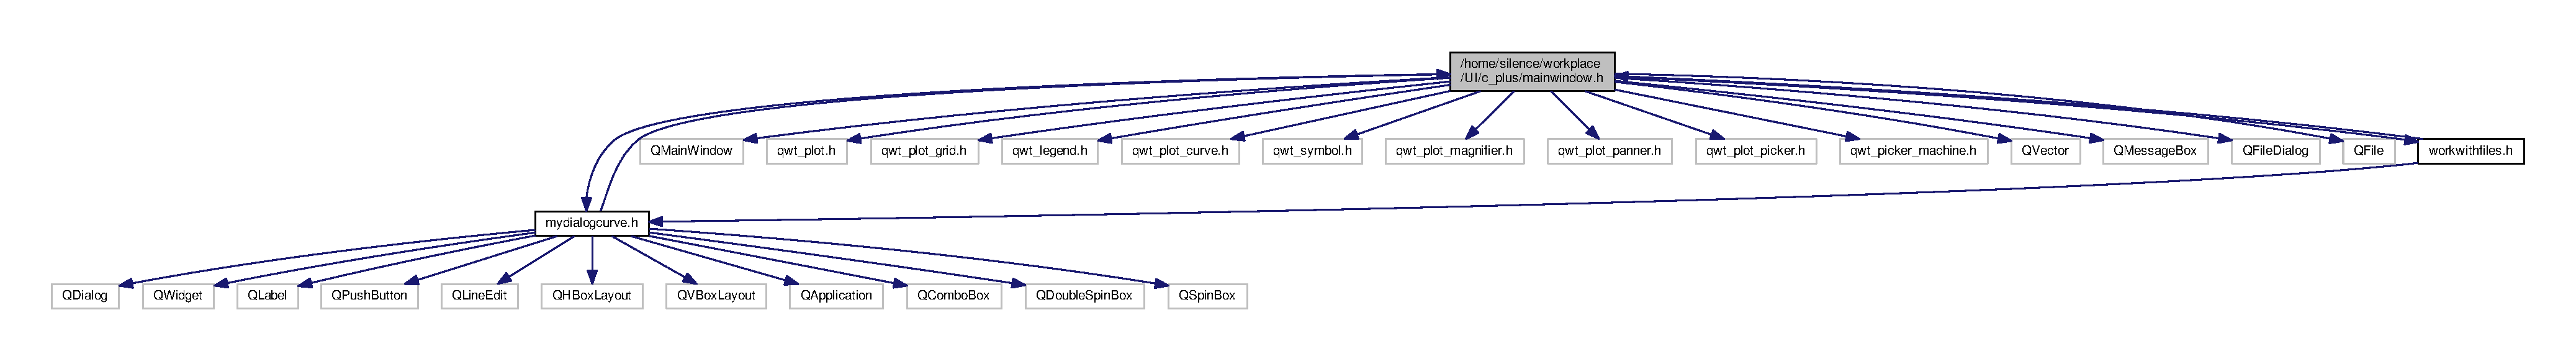
\includegraphics[width=350pt]{mainwindow_8h__incl}
\end{center}
\end{figure}
Граф файлов, в которые включается этот файл\+:\nopagebreak
\begin{figure}[H]
\begin{center}
\leavevmode
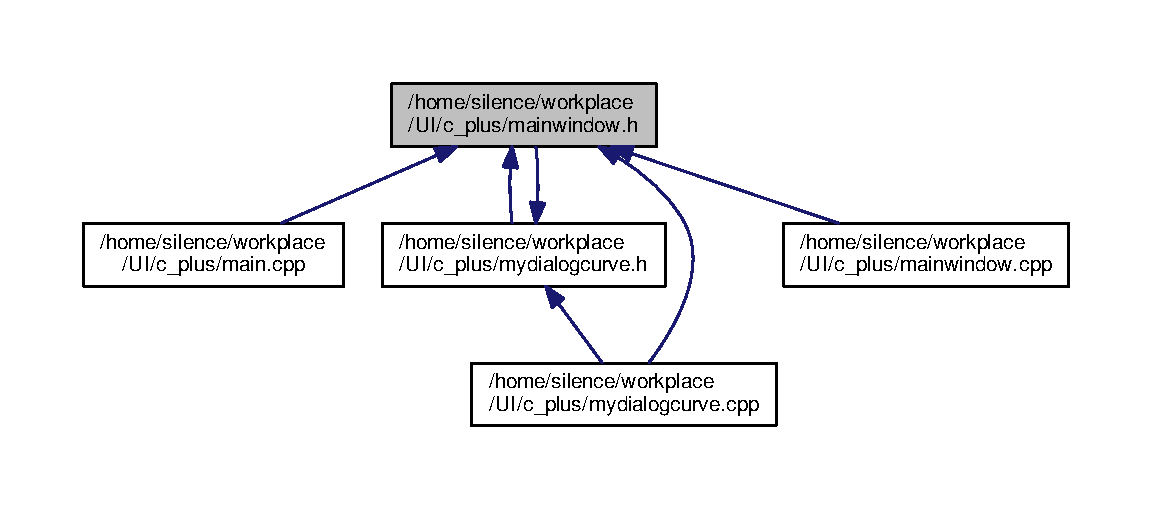
\includegraphics[width=350pt]{mainwindow_8h__dep__incl}
\end{center}
\end{figure}
\subsection*{Классы}
\begin{DoxyCompactItemize}
\item 
class \hyperlink{classgraph}{graph}
\begin{DoxyCompactList}\small\item\em The graph class. \end{DoxyCompactList}\item 
class \hyperlink{class_main_window}{Main\+Window}
\begin{DoxyCompactList}\small\item\em The \hyperlink{class_main_window}{Main\+Window} class. \end{DoxyCompactList}\end{DoxyCompactItemize}


\subsection{Подробное описание}
Загловочный файл содержащий класс прямой и главное окно , в котором и рисуются прямые 

Содержит описание класса графиков, главного окна 
\hypertarget{mydialogcurve_8h}{}\section{Файл /home/silence/workplace/\+U\+I/c\+\_\+plus/mydialogcurve.h}
\label{mydialogcurve_8h}\index{/home/silence/workplace/\+U\+I/c\+\_\+plus/mydialogcurve.\+h@{/home/silence/workplace/\+U\+I/c\+\_\+plus/mydialogcurve.\+h}}


Загловочный файл окон добавления и удаления графиков  


{\ttfamily \#include \char`\"{}mainwindow.\+h\char`\"{}}\\*
{\ttfamily \#include $<$Q\+Dialog$>$}\\*
{\ttfamily \#include $<$Q\+Widget$>$}\\*
{\ttfamily \#include $<$Q\+Label$>$}\\*
{\ttfamily \#include $<$Q\+Push\+Button$>$}\\*
{\ttfamily \#include $<$Q\+Line\+Edit$>$}\\*
{\ttfamily \#include $<$Q\+H\+Box\+Layout$>$}\\*
{\ttfamily \#include $<$Q\+V\+Box\+Layout$>$}\\*
{\ttfamily \#include $<$Q\+Application$>$}\\*
{\ttfamily \#include $<$Q\+Combo\+Box$>$}\\*
{\ttfamily \#include $<$Q\+Double\+Spin\+Box$>$}\\*
{\ttfamily \#include $<$Q\+Spin\+Box$>$}\\*
Граф включаемых заголовочных файлов для mydialogcurve.\+h\+:\nopagebreak
\begin{figure}[H]
\begin{center}
\leavevmode
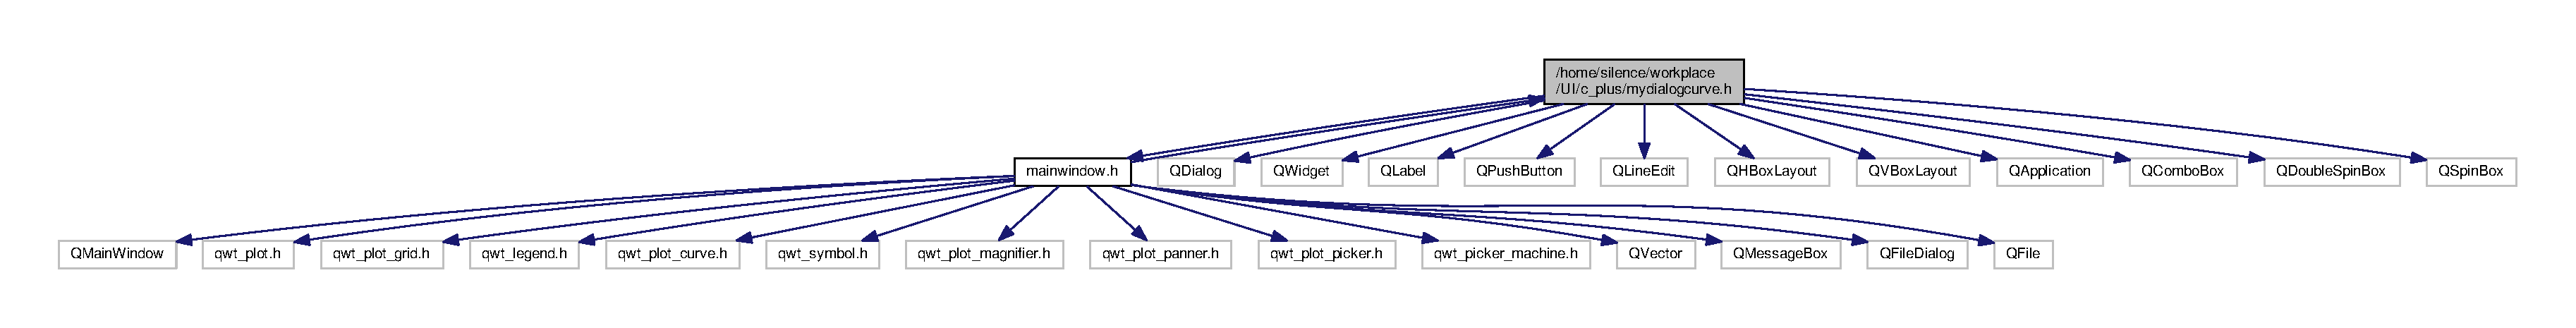
\includegraphics[width=350pt]{mydialogcurve_8h__incl}
\end{center}
\end{figure}
Граф файлов, в которые включается этот файл\+:\nopagebreak
\begin{figure}[H]
\begin{center}
\leavevmode
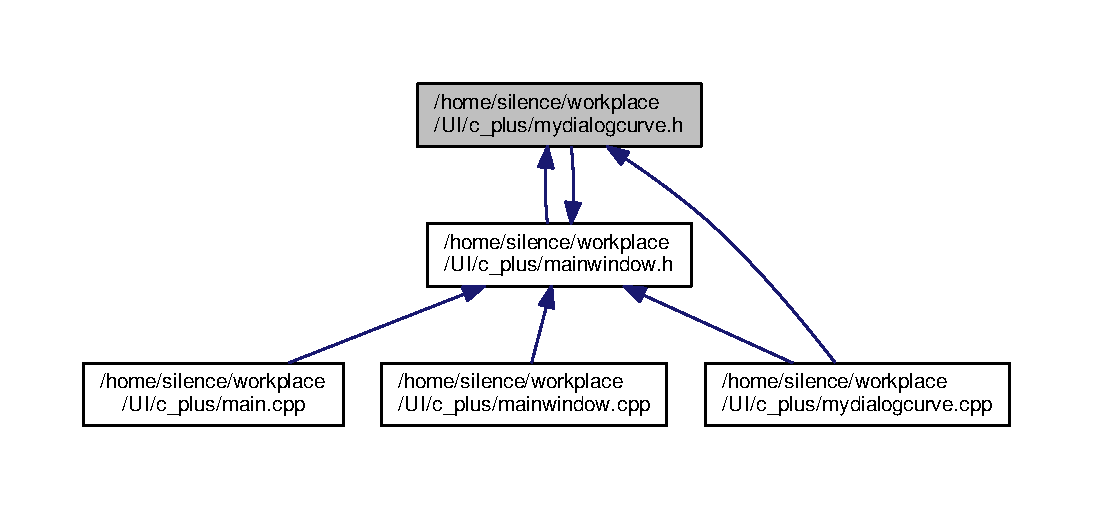
\includegraphics[width=350pt]{mydialogcurve_8h__dep__incl}
\end{center}
\end{figure}
\subsection*{Классы}
\begin{DoxyCompactItemize}
\item 
class \hyperlink{class_my_new_curve}{My\+New\+Curve}
\begin{DoxyCompactList}\small\item\em The \hyperlink{class_my_new_curve}{My\+New\+Curve} class. \end{DoxyCompactList}\item 
class \hyperlink{class_my_delete_curve}{My\+Delete\+Curve}
\begin{DoxyCompactList}\small\item\em The \hyperlink{class_my_delete_curve}{My\+Delete\+Curve} class. \end{DoxyCompactList}\end{DoxyCompactItemize}


\subsection{Подробное описание}
Загловочный файл окон добавления и удаления графиков 

Содержит в себе описания двух окон добавления и удаления 
\hypertarget{workwithfiles_8h}{}\section{Файл /home/silence/workplace/\+U\+I/c\+\_\+plus/workwithfiles.h}
\label{workwithfiles_8h}\index{/home/silence/workplace/\+U\+I/c\+\_\+plus/workwithfiles.\+h@{/home/silence/workplace/\+U\+I/c\+\_\+plus/workwithfiles.\+h}}


Загловочный файл содержащий классы работы с файлами  


{\ttfamily \#include \char`\"{}mainwindow.\+h\char`\"{}}\\*
{\ttfamily \#include \char`\"{}mydialogcurve.\+h\char`\"{}}\\*
Граф включаемых заголовочных файлов для workwithfiles.\+h\+:\nopagebreak
\begin{figure}[H]
\begin{center}
\leavevmode
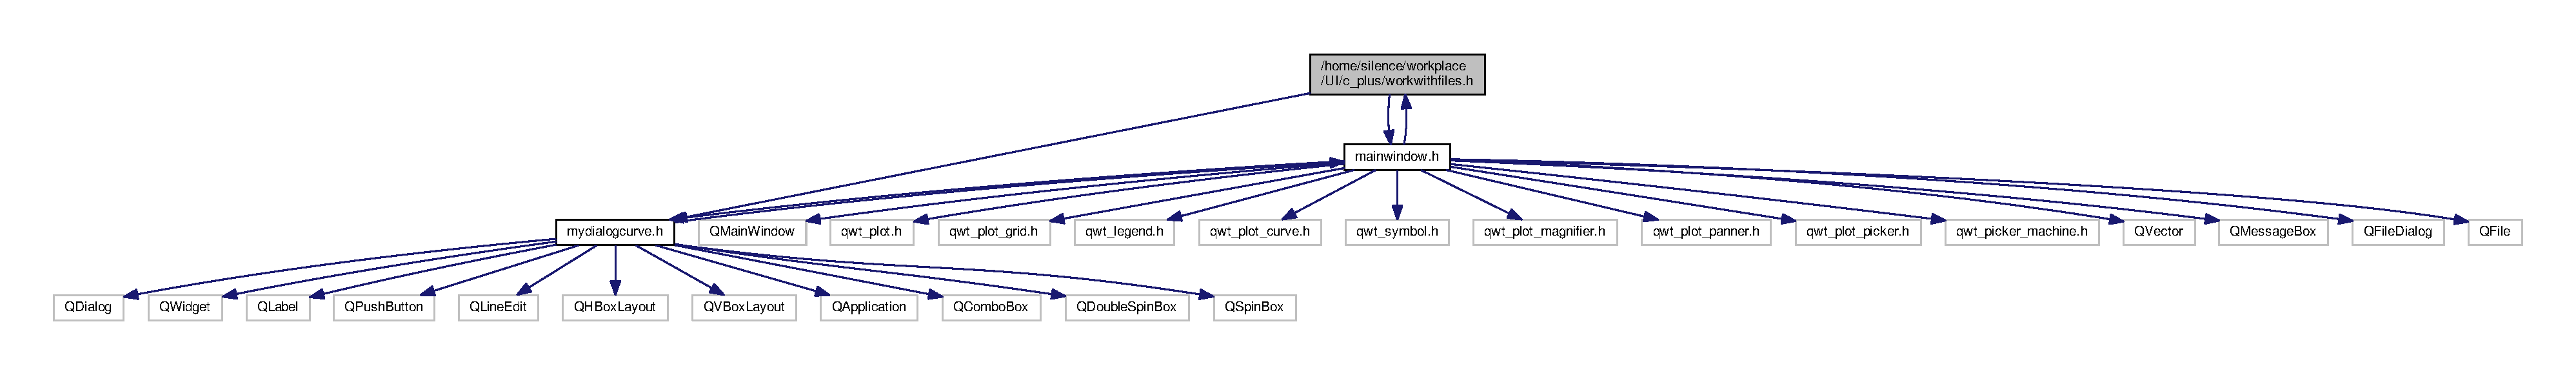
\includegraphics[width=350pt]{workwithfiles_8h__incl}
\end{center}
\end{figure}
Граф файлов, в которые включается этот файл\+:\nopagebreak
\begin{figure}[H]
\begin{center}
\leavevmode
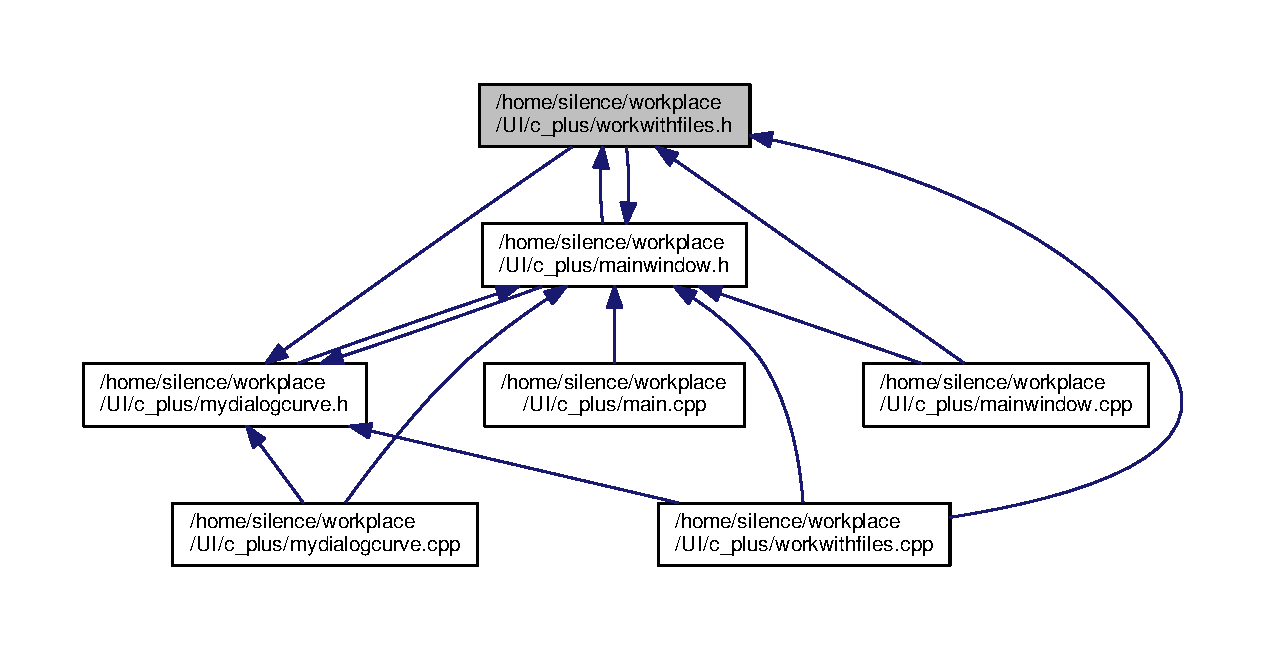
\includegraphics[width=350pt]{workwithfiles_8h__dep__incl}
\end{center}
\end{figure}
\subsection*{Классы}
\begin{DoxyCompactItemize}
\item 
class \hyperlink{class_format_factory}{Format\+Factory}
\begin{DoxyCompactList}\small\item\em The \hyperlink{class_format_factory}{Format\+Factory} class. \end{DoxyCompactList}\item 
class \hyperlink{class_txt}{Txt}
\begin{DoxyCompactList}\small\item\em Класс для работы с .txt форматом \end{DoxyCompactList}\item 
class \hyperlink{class_doc}{Doc}
\begin{DoxyCompactList}\small\item\em Класс для работы с .doc форматом \end{DoxyCompactList}\end{DoxyCompactItemize}


\subsection{Подробное описание}
Загловочный файл содержащий классы работы с файлами 

class \hyperlink{class_format_factory}{Format\+Factory} является абстрактным и используется только для наследования. 
%--- End generated contents ---

% Index
\backmatter
\newpage
\phantomsection
\clearemptydoublepage
\addcontentsline{toc}{chapter}{Алфавитный указатель}
\printindex

\end{document}
